\chapter{Design and Implementation}
\label{chap:design_and_implementation}

In this chapter, we will discuss the design and implementation of the \ac{POP} algorithm, the design of the Virtual Environment  and the Unity components that were used to visualize the \ac{POP} algorithm. The chapter will also discuss the design of the user interface and the interaction techniques that were used in the \ac{VR} game.

\section[POP Algorithm]{\ac{POP} Algorithm} \label{sec:pop_algorithm_design}

This section will discuss some of the design decisions that were made during the implementation of the \ac{POP} algorithm. It will include an overview of the implemented algorithms that were used beside the \ac{POP} algorithm. In addition, it will discuss the data structures that were used to represent the planning domain and the planning problem.

\subsection{Nondeterministic Achievers \& Threat Search} \label {subsec:nondeterministic_achievers_threat_search}
\acf{POP} needs to be able to handle some form of nondeterminism in the planning domain. This is because the planner needs
to be able to handle situations where there are multiple ways to achieve a precondition
of an action. Nondeterminism is a concept that is used in computer science to describe the occurrence of events without a predictable outcome, where multiple outcomes are possible from a given state. In the context of planning, nondeterminism is used to describe the situation where there are multiple ways to achieve a precondition of an action, for example.
This cannot be achieved in practice without trying to search all possible ways of the choices that can be made.
So, to model nondeterminism in the planning domain, we need to use some form of graph search algorithm to search for all possible ways to achieve a precondition of an action efficiently. In this project, multiple graph search algorithms were implemented to handle nondeterminism in the planning domain. These algorithms are \ac{A*} Search, \ac{BFS}, and \ac{DLS} which is a variation of \ac{DFS}. All of these algorithms are discussed in detail in the following sections.


\subsection{Graph Search Algorithms} \label{subsec:graph_search_algorithms}
Graph search algorithms are widely used in computer science to solve problems that can be represented as graphs. They have many applications in various fields such as artificial intelligence, computer graphics, and computer vision. In this project, graph search algorithms were used to solve the problem of nondeterminism in the planning domain.
The following graph search algorithms were implemented in the project:
\begin{itemize}

    \item \textbf{\acf{A*} Search Algorithm} \label{subsubsec:a_star} \\
          \ac{A*} Search is a graph search \& traversal algorithm that is widely used in computer science due to its efficiency, optimality, and completeness. It is an informed search algorithm that uses a heuristic function to estimate the cost of reaching the goal from a given state. The heuristic function is used to guide the search towards the goal state by selecting the most promising nodes to explore. \ac{A*} Search is an extension of Dijkstra's algorithm that uses a heuristic function to estimate the cost of reaching the goal from a given state\cite{AStarAlgorithm}. \ac{A*} is a Best First Search algorithm that uses a priority queue to store the nodes to be explored. The priority queue is ordered based on a cost function that combines the cost of reaching the node from the start state and the heuristic estimate of the cost of reaching the goal from the node. The cost function is defined as $f(n) = g(n) + h(n)$, where $g(n)$ is the cost of reaching the node from the start state and $h(n)$ is the heuristic estimate of the cost of reaching the goal from the node. The algorithm selects the node with the lowest $f$ value from the priority queue and explores its neighbors until the goal is reached. The algorithm is guaranteed to find the optimal solution if the heuristic function is admissible, i.e., it never overestimates the cost of reaching the goal from a given state. The algorithm is also complete if the search space is finite and the heuristic function is consistent.

          In this project, $g(n)$ is the path (level) cost from the root node to the current node, and $h(n)$ heuristic was chosen to be the number of unsatisfied preconditions, i.e., the count of pairs in the $agenda$ discussed in section {\ref{subsec:pop_algorithm}}.

    \item \textbf{\acf{DLS} Search Algorithm} \label{subsubsec:dls}\\
          First, let's discuss the \ac{DFS} algorithm.
          \ac{DFS} is an uninformed search algorithm that is widely used in computer science to explore a graph or tree data structure. It is a depth-first traversal algorithm that explores the nodes deep in the graph before exploring the nodes at the same level. The algorithm starts at the root node and explores the nodes along each branch before backtracking to explore the other branches. The algorithm uses a stack data structure to store the nodes to be explored. The algorithm is not guaranteed to find the optimal solution, but it is complete if the search space is finite. The algorithm is also efficient in terms of memory usage as it only needs to store the nodes along the current path. However, the algorithm can get stuck in infinite loops if the graph contains an infinite deep path. To avoid this problem, a depth limit can be imposed on the search to limit the depth of the search tree. This is known as the \acf{DLS} algorithm. The algorithm is similar to \ac{DFS} but with an additional depth limit parameter that specifies the maximum depth of the search tree. The algorithm stops exploring a branch when the depth limit is reached and backtracks to explore other branches. The algorithm is complete if the depth limit is greater than the depth of the optimal solution. The algorithm is also efficient in terms of memory usage. In this project, \ac{DLS} was also provided as an option to be used in the \ac{POP} algorithm.

    \item \textbf{\acf{BFS} Search Algorithm} \label{subsubsec:bfs}\\
          \ac{BFS} is an uninformed search algorithm that is widely used to explore a graph or tree data structure. It is a breadth-first traversal algorithm, meaning that it explores the nodes at the same level before exploring the nodes at the next level. The algorithm starts at the root node and explores the nodes at the same level before moving to the next level. The algorithm uses a queue data structure to store the nodes to be explored. The algorithm is guaranteed to find a solution if one exist, even if the graph is infinite. However, the algorithm is not guaranteed to always find the optimal solution. The algorithm is also inefficient in terms of memory usage as it needs to store all the nodes at the current level. In this project, \ac{BFS} was also provided as an option to be used in the \ac{POP} algorithm.

\end{itemize}

\subsection{Unification Algorithm} \label{subsec:unification_algorithm}
Finding the \acf{MGU} of two terms is a crucial step in the \ac{POP} algorithm. The \ac{MGU} is used to unify two terms by finding a substitution that makes the two terms equal. The \ac{MGU} is the most general substitution that can be applied to the two terms to make them equal.
For example, consider the following terms: $P(x, B)$ and $P(A, y)$. The \ac{MGU} of these two terms is $\{x/A, y/B\}$, which means that the terms can be unified by substituting $A$ for $x$ and $B$ for $y$ to make them equal to $P(A, B)$.
The \ac{MGU} is used to unify the preconditions of an action with the current state of the world to determine if the action can be applied. The \ac{MGU} is also used to unify the effects of an action that can be used, for example, to detect threats in the partial plan.

In this project, the \ac{MGU} algorithm was implemented using a variation of the unification algorithm discussed in Russell and Norvig's book in Chapter 9 \cite{RN2009_Ch.9}, and taken from the lecture slides of the course \textit{Introduction to Artificial Intelligence} by Prof. Haythem Ismail \cite{Ismail2023}.
There is a convention used in the algorithm implementation: the variables are represented as strings starting with a lowercase letter, and the constants are represented as strings starting with an uppercase letter.
The algorithm described in \autoref{alg:unification_algorithm} has three main functions: UNIFY, UNIFY1, and UNIFYVAR. The UNIFY function takes two expressions as input, listifies them, and then calls the UNIFY1 function with the two listified expressions and an empty substitution set. An example of listifying an expression is converting the expression $P(x, f(y,z))$ to the list $[P, x, [f, y, z]]$.
\begin{algorithm}[H]
    \caption{Unification Algorithm}
    \begin{algorithmic}[1]
        \label{alg:unification_algorithm}
        \STATE \textbf{function} UNIFY($E1, E2$) :
        \RETURN UNIFY1(LISTIFY($E1$), LISTIFY($E2$), $\{\}$);
        \STATE
        --------------------------------------------------------------------------------------------------------
        \STATE
        \STATE \textbf{function} UNIFY1($E1, E2, \mu$) :
        \IF{$\mu = \text{fail}$}
        \RETURN fail
        \ENDIF
        \IF{$E1 = E2$}
        \RETURN $\mu$
        \ENDIF
        \IF{VAR?($E1$)}
        \RETURN UNIFYVAR($E1, E2, \mu$)\ENDIF
        \IF{VAR?($E2$)}
        \RETURN UNIFYVAR($E2, E1, \mu$)
        \ENDIF
        \IF{ATOM?($E1$) or ATOM?($E2$)}
        \RETURN fail
        \ENDIF
        \IF{LENGTH($E1$) != LENGTH($E2$)}
        \RETURN fail
        \ENDIF
        \RETURN UNIFY1(REST($E1$), REST($E2$), UNIFY1(FIRST($E1$), FIRST($E2$), $\mu$))
        \STATE
        --------------------------------------------------------------------------------------------------------
        \STATE
        \STATE \textbf{function} UNIFYVAR($x, e, \mu$) :
        \IF{$t/x \in \mu$ and $t \neq x$}
        \RETURN UNIFY1($t, e, \mu$)
        \ENDIF
        \STATE $t = \text{SUBST}(\mu, e)$
        \IF{$x$ occurs in $t$}
        \RETURN fail
        \ELSE
        \RETURN $\mu \circ \{t/x\}$
        \ENDIF
    \end{algorithmic}
\end{algorithm}
The UNIFY1 function takes two listified expressions and a substitution set as input and returns the most general unifier of the two expressions. The UNIFYVAR function takes a variable, an expression, and a substitution set as input and returns the most general unifier of the variable and the expression. The main algorithm starts in line 6 by checking if the substitution set is a failure, in which it returns a failure. Then, it checks if the two expressions are equal, in which it returns the current substitution set. Then, it checks if $E1$ or $E2$ is a variable, in which it calls the UNIFYVAR function with the first parameter being the variable and the second parameter being the expression. Then, it checks if $E1$ or $E2$ is an atom, in which it returns a failure in line 19. The reason for this is that after making sure that neither $E1$ nor $E2$ are variables, and they are not equal, then they must be different atoms, and thus cannot be unified. Then, it checks if the length of $E1$ is not equal to the length of $E2$, in which it returns a failure in line 22, as we cannot unify two expressions with different lengths, like $P(x)$ and $P(x, y)$. Finally, it calls the UNIFY1 function recursively with the rest of the two expressions and the unification of the first elements of the two expressions.

The UNIFYVAR function starts by checking if the variable $x$ is already in the substitution set and bound to a term $t$ that is not equal to $x$, in which it calls the UNIFY1 function with the term $t$ and the input expression $e$. If the variable $x$ is not in the substitution set, then it substitutes every term in the expression $e$ with the substitution set $\mu$. Then, it checks if the variable $x$ occurs in the term $t$, in which it returns a failure, as we cannot unify a variable with an expression that contains the variable. If we had $x$ and $f(x)$, then the unification would fail, since it would result in an infinite recursion.
Otherwise, it returns the substitution set $\mu$ composite with the substitution $\{t/x\}$, which means that the term $t$ is substituted for the variable $x$ in the substitution set $\mu$.

\begin {figure}[h]
\dirtree{%
    .1 /POP.
    .2 controller.
    .3 POPController.cs.
    .2 engine.
    .3 Action.cs.
    .3 Agenda.cs.
    .3 BindingConstraints.cs.
    .3 CausalLink.cs.
    .3 Helpers.cs.
    .3 Literal.cs.
    .3 Operator.cs.
    .3 ParitalPlan.cs.
    .3 Planner.cs.
    .3 PlanningProblem.cs.
    .3 PriorityQ.cs.
}
\caption{Folder Structure of the POP Algorithm Engine}
\label{fig:pop_folder_structure}
\end{figure}


\subsection{Classes and Folder Structure} \label{subsec:class_diagram_and_folder_structure}
The \ac{POP} algorithm engine was implemented in C\#. The algorithm engine was divided into two main folders: the controller folder and the engine folder. The folder structure of the \ac{POP} algorithm engine is shown in \autoref{fig:pop_folder_structure}. The controller folder contains the \textbf{POPController} class, which is responsible for controlling the execution of the \ac{POP} algorithm for Unity. The engine folder contains all the classes that implement the \ac{POP} algorithm.
The class diagram of the \ac{POP} algorithm presented in \autoref{fig:pop} shows the main classes and their relationships in the \ac{POP} algorithm. In the following list, we will discuss the main classes, their responsibilities, how they are implemented, and what their structure is:
\begin{itemize}
    \item \textbf{PlanningProblem Class:} \\
          The \textbf{PlanningProblem} class is responsible for representing the planning problem, that is the only input to the \acl{POP} algorithm. The \textbf{PlanningProblem} class has the initial state, the goal state, and the set of operators as its members. The initial and goal states are represented as list of \textit{Literal} objects. The operators are represented as a list of \textit{Operator} objects. The class keeps hold of a list of \textit{Literals}, that is not given as an input, but is instantiated automatically once the planning problem is initialized, and it is used to keep track of the existing literals from the initial and goal states in addition to the literals in the preconditions and effects of the operators. This list is to assist the planner.

          The class has only one functional method, which is the \textbf{GetListOfAchievers()} method, that takes a \textit{literal} as input. The \textbf{GetListOfAchievers()} method is responsible for returning a list of operators that can achieve the input \textit{literal}. The \textbf{PlanningProblem} class also has some predefined problems that can be used to test the \ac{POP} algorithm and the \ac{VR} game. Among these problems are the \textit{Socks and Shoes problem}, the \textit{Milk, Bananas, and Cordless Drill problem}, the \textit{Groceries Buying problem} which is a simplified variation of the \textit{Milk, Bananas, and Cordless Drill problem}, and some other problems.

    \item \textbf{PartialPlan Class:} \\
          The \textbf{PartialPlan} class is responsible for representing the partial plan that is being constructed by the \ac{POP} algorithm. The \textbf{PartialPlan} class has a set of actions, a set of causal links, an instance of \textit{BindingConstraints} object, and a set of ordering constraints as its members. The class contains some helper functions that are used by the planner like the \textit{GetListOfActionAchievers()} method, and some others that are shown in the class diagram in \autoref{fig:pop}.

    \item \textbf{Planner Class:} \\
          It is the main class that has the core logic of the \ac{POP} algorithm. The \textbf{Planner} class has the Planning Problem, the Partial Plan, and the Agenda as its members. It also has variables counter array to keep track of the generated distinct variables. The following list will discuss the logic and flow of the \ac{POP} algorithm in the \textbf{Planner} class:
          \begin{itemize}
              \item The \textbf{Planner} class has the \textit{POP()} method that implements the \ac{POP} algorithm. The \textit{POP()} method is responsible for generating the plan by creating a priority queue or stack to store nodes to be used while searching. The \textit{POP()} method also has a loop that iterates over the priority queue or stack until the goal is reached or no nodes are left.
                    For each node, it checks if the node partial plan is not acyclic, if it is not, then it pops the node from the priority queue or stack and continues to the next node. If the partial plan is acyclic, then it checks if the node is a goal node, if it is, then it returns the plan. If the node is not a goal node, then it expands the node by applying the applicable actions to the node.

                    % image of the pop class diagram (POP.png)
                    \begin{figure}[H]
                        \centering
                        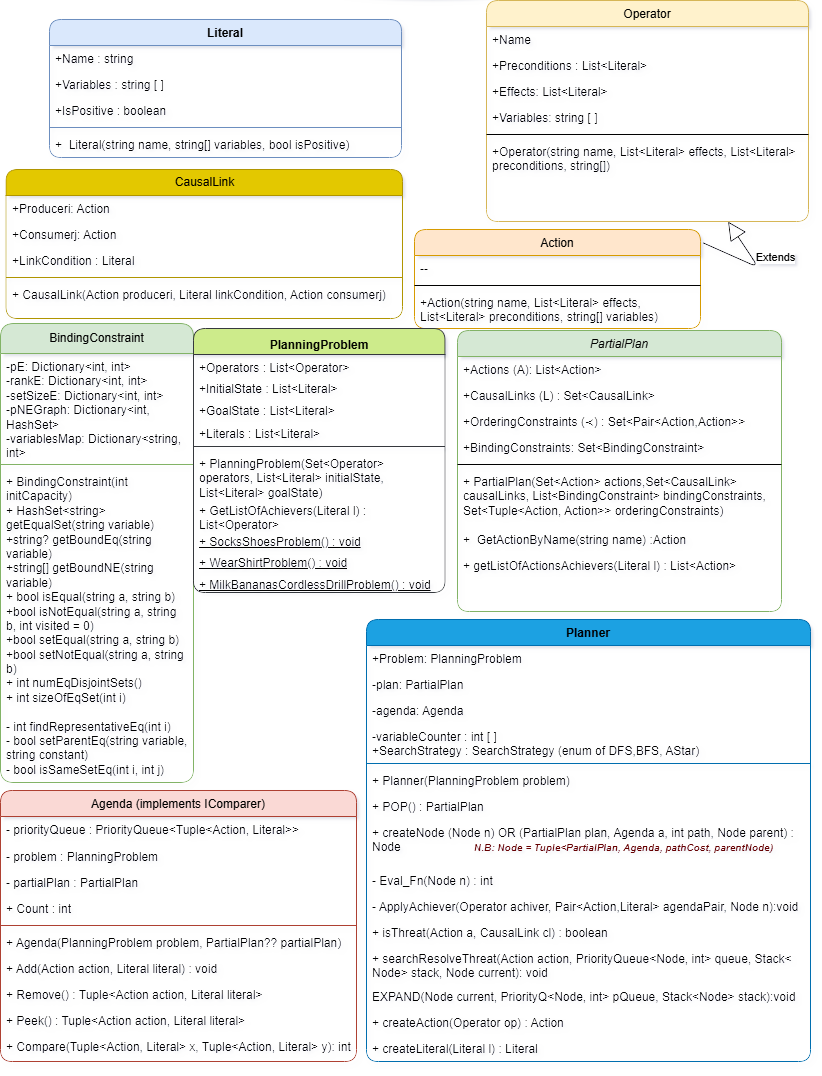
\includegraphics[width=0.8\textwidth]{images/POP.png}
                        \caption[Class Diagram of the POP Algorithm]{Class Diagram of the POP Algorithm}
                        \label{fig:pop}
                    \end{figure}
              \item The \textit{EXPAND()} method is responsible for expanding the node. It first chooses a pair of ($action$, $precondition$) from the $agenda$ based on some heuristic. The heuristic that I chose is to prioritize the pair with the precondition that has the least number of achievers, and this will be discussed in more details later in this section in the \textbf{Agenda} class implementation. Then, after selecting a pair of ($action$, $precondition$), the \textit{POP()} method gets the achievers by gathering the existing actions and new operators that can achieve this precondition, and for each achiever, it creates a new node applies this achiever to it and then adds this node to the main queue or stack.

              \item The \textbf{POP} method also has a helper method called \textit{ApplyAchiever()} that applies the achiever to the node. The \textit{ApplyAchiever()} method works by unifying the achiever's effect with the precondition of the action, then it adds the binding constraints to the partial plan of the node, and then it adds the causal link to the partial plan, as well as updating the ordering constraints with the achiever being ordered before the action with the precondition we are trying to achieve. It also checks whether the achiever is an existing action or a new action, so that if it is a new action, it adds it to the partial plan, update its ordering constraints to be between the \textit{Start} and \textit{Finish} actions, and adds the new action's preconditions to the agenda.

              \item After applying the achiever, the \textit{EXPAND()} method checks if the new node has threats before adding it to the priority queue or stack through a helper function, \textit{searchResolveThreats()}. The \textit{searchResolveThreats()} method is responsible for searching for threats in the partial plan and resolving them recursively until no threats are left. The \textit{searchResolveThreats()} method has the new added action achiever and the new causal link as inputs. It first starts to check if any of the causal links in the partial plan is threatened by the new action, and if it is, then it resolves the threat by trying promotion and demotion on new cloned nodes. If no other threats are found, then the new node is added to the priority queue or stack.

              \item The \textit{searchResolveThreats()} method also has a helper method called \textit{isThreat()} that checks if a causal link is threatened by an action. The \textit{isThreat()} method works by checking the conditions, discussed in the definition in Section \ref{def:threat}, to be a threat. The \textit{searchResolveThreats()} then checks if the new causal link input is threatened by any of the existing actions in the partial plan. If it is, then it follows the same steps as before to resolve the threat until there is no threats.

              \item No node is added to the main queue or stack until it passes all the checks and has no threats. All nodes outputted from the resolving of threats caused by the new action are then passed to checking whether the new causal link is threatened by any other action. After extensive testing, the planner was found to output wrong results of the all threats are not resolved recursively, or through an iterative approach of the recursive method, as this is the only stage where threats are checked and resolved.
          \end{itemize}

    \item \textbf{Agenda Class:} \\
          The \textbf{Agenda} class is responsible for representing the agenda that is used by the \ac{POP} algorithm. The agenda is a list of pairs of ($action$, $precondition$) that are used to keep track of the preconditions that need to be achieved. The class internally uses a priority queue to store the pairs of ($action$, $precondition$). The chosen heuristic is to prioritize the pair with the precondition that has the least number of achievers. This is because the precondition with the least number of achievers minimizes the branching factor of the search tree, which leads to a more efficient search \cite{RN2020_Ch.11}. This leads to detecting special cases faster, like the case where the precondition has only one achiever, in which the planner has no any other choice but to apply this achiever. The \textbf{Agenda} class has a custom comparer method that compares with the number of achievers of the preconditions. Finally, in the special case where the number of achievers is zero, the class throws an exception, indicating that there is no solution to the problem, and something is wrong with the input problem.

    \item \textbf{Operator Class:} \\
          The \textbf{Operator} class is responsible for representing the operators that are used in the planning domain. The operators has a name, a list of preconditions, a list of effects, and a string variables array to represent the unbonded variables and their relations in the effects and the preconditions of the operator.

    \item \textbf{Action Class:} \\
          The \textbf{Action} class is responsible for representing the actions that are used in the partial plan. The \textit{Operator} class is the superclass of this class. The \textbf{Action} class inherits the name, preconditions, effects, and variables array from the \textit{Operator} class. The class also has a method that checks if the action has conflicts in the effects or the preconditions. The conflicts that \textit{hasConflictingPreconditionsOrEffects()} method checks is of of that format: for example if $P(x), \lnot P(y) \in \text{preconditions}$, where $x$ and $y$ are bound to the same variable, and $P$ is the same predicate. This is a conflict because it is impossible for $x$ and $y$ to be the same variable and different at the same time.

    \item \textbf{Literal Class:} \\
          The \textbf{Literal} class is responsible for representing the literals, the conditions or the predicates that are used in the planning domain. The literals, in this project, are used to represent the preconditions, the effects, the initial state, and the goal state. The \textbf{Literal} class has a name, a list of arguments, and a boolean variable to represent the negation of the literal.

    \item \textbf{BindingConstraints Class:} \\
          The \textbf{BindingConstraints} class is responsible for representing the binding constraints that are used in the partial plan. The binding constraints contains all variables that are bound and equal (or not equal) to a constant term or another variable. As mentioned in \autoref{subsec:unification_algorithm}, there is a convention that variables are lowercase strings and constants are uppercase strings.
          In this class, the focus os on four main methods: \textit{SetEqual()}, \textit{SetNotEqual()}, \textit{getBoundEq()}, and \textit{getBoundNE()}. The \textit{SetEqual()} and \textit{SetNotEqual()} methods are used to set the constraints of the variables to be equal or not equal to each other. The \textit{getBoundEq()} and \textit{getBoundNE()} methods are used to get the variables that are bound equal or not equal to a term or another variable.

          In this project, for the \textbf{non-equality constraints}, I used a regular \textit{Hash Map} or \textit{Dictionary} data structure to store the constraints. The key of the \textit{Dictionary} is the variable, and the value is a list of variables not equal to the key variable. There is no relation between the variables in the list, and the list is not ordered.

          As for the \textbf{equality constraints} between the variables, I used a \textit{Disjoint Sets} representation. \textbf{Disjoint Sets} data structure is a set of elements partitioned into a number of non-overlapping subsets\cite{WikiDisjointSet}\cite{GeeksForGeeksDisjointSet}. The main reason for using a \textit{Disjoint Set} is that it is efficient in terms of time complexity. The implementation used in this project uses the \textit{Union-Find} algorithm to merge the sets and find the representative of the set, in other words, the constant term that is bound to the variable, or a variable if no constant term is bound to it. The \textit{Union-Find} implementation guarantees a time complexity of $O(\log n)$, where $n$ is the number of variables in the partial plan. This number may be large for some problems as the planner uses an incremented counter to generate new variables in action's parameters, as well as in the effects and preconditions of the actions. This number continues to grow as the planner decides to backtrack and generate new actions. Besides the time complexity, the \textit{Disjoint Set} was chosen because for all equal variables in a set, it will always have the same root, which is the representative of the set, which can make things easier to trace for humans.

          Using both data structures, the \textit{Dictionary} and the \textit{Disjoint Set}, the planner can easily check if there exists some logical contradiction in the binding constraints. For example, if there is a variable $x$ that is bound equal to a variable $y$, and $y$ is bound equal to a third variable $z$, then another constraint that makes $x$ not equal to $z$ is added directly or indirectly, then the \textbf{BindingConstraints} class can easily detect this contradiction and stop the search.

    \item \textbf{CausalLink Class:} \\
          The \textbf{CausalLink} class is responsible for representing the causal links that are used in the partial plan. The exact definition of a causal link is discussed in the definition in Section \ref{def:causal_link}. The \textbf{CausalLink} class has a \textit{LinkCondition} of type \textit{Literal}, a \textit{Produceri} of type \textit{Action}, and a \textit{Consumerj} of type \textit{Action}.
          The \textit{Produceri} is the action that has the effect that is the \textit{LinkCondition}, and the \textit{Consumerj} is the action that has the precondition that is also the \textit{LinkCondition}.

    \item \textbf{PriorityQ Class:} \\
          The \textbf{PriorityQ} is a class taken from the Microsoft documentation and GitHub repository under the MIT license\cite{MicrosoftPQ}\cite{GitHubPQ}. The class is used to mimic the internal original implementation of the \textit{PriorityQueue} in C\#. The reason for creating this class is that the latest Unity \ac{LTS} version at the time of writing this thesis uses an older version of C\# language (C\# 9.0) that does not have the \textit{PriorityQueue} class.

\end{itemize}


% showing the results and outputs of running the code
\subsection{POP Terminal Output} \label{subsec:pop_output}

The \ac{POP} algorithm was tested using the \textit{Socks and Shoes problem}, the \textit{Milk, Bananas, and Cordless Drill problem}, the \textit{Groceries Buying problem}, the \textit{Spare Tires problem}, and some other custom problems. The \ac{POP} algorithm was able to find the optimal solution for all the problems that were tested. Next, we will show the output for the \textit{Milk, Bananas, and Cordless Drill problem} and the \textit{Spare Tires problem}.

\subsubsection{Milk, Bananas, and Cordless Drill Problem} \label{subsubsec:milk_bananas_cordless_drill_output}
The \textit{Milk, Bananas, and Cordless Drill problem} is a problem where the agent needs to buy milk and bananas from the supermarket and go to the hardware store to buy a cordless drill. Now let's see the input to the planner in \autoref{code:milk_bananas_cordless_drill_input}:

% code snippet of the input to the planner
\begin{lstlisting}[language={[Sharp]C}, frame=single, basicstyle=\small\ttfamily, breaklines=true, captionpos=b, caption={Milk, Bananas, and Cordless Drill Problem Input to the Planner}, label={code:milk_bananas_cordless_drill_input}]
PlanningProblem milkBananasCordlessDrill = new PlanningProblem(
    operators: new HashSet<Operator> {
        new Operator("Buy", variables: new []   { "x" },
            preconditions: new List<Literal> { new ("Sells", new[]{ "store", "x" }), new ("At",new[]{ "store" }) },
            effects:     new List<Literal> { new ("Have", new[]{"x"}) }
        ),
        new Operator("Go", variables: new[]   { "there" },
            preconditions:  new List<Literal> { new ("At", new[]{ "here" }),       new ("At", new[]{"there"}, false) },
            effects:        new List<Literal> { new ("At", new[]{ "here" }, false), new ("At", new[]{"there"}) }
        )
    },
    initialState: new List<Literal>{ new("At",new []{"Home"}), new("Sells", new []{"SM", "Milk"}), new("Sells", new []{"SM", "Bananas"}), new("Sells", new []{"HWS", "Drill"})
                    , new("At",new []{"HWS"}, false), new("At", new []{"SM"}, false)},
    goalState: new List<Literal> { new("At", new string[] { "Home" }), new("Have", new[] { "Milk" }), new("Have", new[] { "Bananas" }), new("Have", new[] { "Drill" }) }
);
\end{lstlisting}

The planner was able to find the optimal solution for the \textit{Milk, Bananas, and Cordless Drill problem} in runtime of 00.260 seconds. The output of the planner is shown in \autoref{code:milk_bananas_cordless_drill_output}:

% code snippet of the output of the planner
\begin{lstlisting}[frame=single, basicstyle=\small\ttfamily, breaklines=true, captionpos=b, caption={Milk, Bananas, and Cordless Drill Problem Output of the Planner}, label={code:milk_bananas_cordless_drill_output}]
    Searching.......................................

Plan  found: 


Linearized Steps:
*************
Start() -> Go(HWS) -> Buy(Drill) -> Go(SM) -> Buy(Bananas) -> Buy(Milk) -> Go(Home) -> Finish()
************

Actions: Start(), Finish(), Go(Home), Buy(Drill), Buy(Milk), Go(SM), Buy(Bananas), Go(HWS)

Links: 
Go(Home) --At(Home)--> Finish(), 
Buy(Drill) --Have(Drill)--> Finish(), 
Start() --Sells(HWS, Drill)--> Buy(Drill), 
Buy(Milk) --Have(Milk)--> Finish(), 
Start() --Sells(SM, Milk)--> Buy(Milk), 
Go(SM) --At(SM)--> Buy(Milk), 
Buy(Bananas) --Have(Bananas)--> Finish(), 
Start() --Sells(SM, Bananas)--> Buy(Bananas), 
Go(SM) --At(SM)--> Buy(Bananas), 
Go(HWS) --At(HWS)--> Go(SM), 
Go(HWS) --At(HWS)--> Buy(Drill), 
Go(SM) --At(SM)--> Go(Home), 
Start() --At(Home)--> Go(HWS), 
Start() -- ¬At(HWS)--> Go(HWS), 
Start() -- ¬At(SM)--> Go(SM), 
Go(HWS) -- ¬At(Home)--> Go(Home)

Binding Constraints: 
{
Equal:
g0 = Home = a4,
b1 = Drill,
s1 = HWS = g4 = a2,
b3 = Milk,
s3 = SM = g2 = s4 = a0,
b4 = Bananas,

Not Equal:
}


Ordering Constraints: (Start() < Finish()), (Start() < Go(Home)), (Go(Home) < Finish()), (Start() < Buy(Drill)), (Buy(Drill) < Finish()), (Start() < Buy(Milk)), (Buy(Milk) < Finish()), (Start() < Go(SM)), (Go(SM) < Finish()), (Go(SM) < Buy(Milk)), (Go(SM) < Go(Home)), (Buy(Milk) < Go(Home)), (Start() < Buy(Bananas)), (Buy(Bananas) < Finish()), (Go(SM) < Buy(Bananas)), (Buy(Bananas) < Go(Home)), (Start() < Go(HWS)), (Go(HWS) < Finish()), (Go(HWS) < Go(SM)), (Go(HWS) < Buy(Drill)), (Buy(Drill) < Go(SM)), (Go(HWS) < Go(Home))

RunTime: 00.260 seconds
\end{lstlisting}

\subsubsection{Spare Tires Problem} \label{subsubsec:spare_tires_output}
The \textit{Spare Tires problem} is a problem where the agent needs to change a flat tire with a spare tire. Now let's see the input to the planner in \autoref{code:spare_tires_input}:

% code snippet of the input to the planner
\begin{lstlisting}[language={[Sharp]C}, frame=single, basicstyle=\small\ttfamily, breaklines=true, captionpos=b, caption={Spare Tires Problem Input to the Planner}, label={code:spare_tires_input}]
PlanningProblem spareTires = new PlanningProblem(
operators: new HashSet<Operator> {
        new Operator("Remove",
            variables:      new []{"obj", "loc"},
            preconditions:  new List<Literal>{ new ("At", new []{"obj", "loc"}), new("Tire", new []{"obj"})},
            effects:        new List<Literal>{ new ("At", new []{"obj", "Ground"}), new("At", new []{"obj", "loc"}, false)}
        ),
        new Operator("PutOn",
            variables:      new []{"t", "Axle"},
            preconditions:  new List<Literal>{ new ("At", new []{"t", "Ground"}), new("At", new []{"Flat", "Axle"}, false), new("Tire", new []{"t"})},
            effects:        new List<Literal>{ new ("At", new []{"t", "Axle"}), new("At", new []{"t", "Ground"}, false)}
        ),
            new Operator("LeaveOvernight",
            variables:      new string []{},
            preconditions:  new(),
            effects:        new List<Literal>{ new ("At", new []{"Spare", "Axle"}, false), new("At", new []{"Spare", "Trunk"}, false), new("At", new []{"Spare", "Ground"}, false)
                    ,new("At", new []{"Flat", "Axle"}, false), new("At", new []{"Flat", "Trunk"}, false), new("At", new []{"Flat", "Ground"}, false)}
        )
    },
initialState: new List<Literal> { new("At", new[] { "Flat", "Axle" }), new("At", new[] { "Spare", "Trunk" }), new("Tire", new[] { "Spare" }), new("Tire", new[] { "Flat" }) },
goalState: new List<Literal> { new("At", new[] { "Spare", "Axle" }), new("At", new[] { "Flat", "Ground" }) }
);
\end{lstlisting}

The planner was able to find the optimal solution for the \textit{Spare Tires problem} in runtime of 00.520 seconds. The output of the planner is shown in \autoref{code:spare_tires_output}:

% code snippet of the output of the planner
\begin{lstlisting}[frame=single, basicstyle=\small\ttfamily, breaklines=true, captionpos=b, caption={Spare Tires Problem Output of the Planner}, label={code:spare_tires_output}]
Searching............

Plan  found: 

Linearized Steps:
*************
Start() -> Remove(Spare, Trunk) -> Remove(Flat, Axle) -> PutOn(Spare, Axle) -> Finish()
************


Actions: Start(), Finish(), PutOn(Spare, Axle), Remove(Flat, Axle), Remove(Spare, Trunk)

Links: 
PutOn(Spare, Axle) --At(Spare, Axle)--> Finish(), 
Start() --Tire(Spare)--> PutOn(Spare, Axle), 
Remove(Flat, Axle) --At(Flat, Ground)--> Finish(), 
Start() --Tire(Flat)--> Remove(Flat, Axle), 
Start() --At(Flat, Axle)--> Remove(Flat, Axle), 
Remove(Spare, Trunk) --At(Spare, Ground)--> PutOn(Spare, Axle), 
Start() --Tire(Spare)--> Remove(Spare, Trunk), 
Start() --At(Spare, Trunk)--> Remove(Spare, Trunk), 
Remove(Flat, Axle) -- ¬At(Flat, Axle)--> PutOn(Spare, Axle)

Binding Constraints: 
{
Equal:
aa1 = Ground,
a2 = Flat = r1,
p0 = Spare = r3,
pp0 = Axle = rr1,
rr3 = Trunk,

Not Equal:
}


Ordering Constraints: (Start() < Finish()), (Start() < PutOn(Spare, Axle)), (PutOn(Spare, Axle) < Finish()), (Start() < Remove(Flat, Axle)), (Remove(Flat, Axle) < Finish()), (Start() < Remove(Spare, Trunk)), (Remove(Spare, Trunk) < Finish()), (Remove(Spare, Trunk) < PutOn(Spare, Axle)), (Remove(Flat, Axle) < PutOn(Spare, Axle))

RunTime: 00.520 seconds
\end{lstlisting}



% --------------------------------------------------------------------------------------------------------------------------------------------------------------------------------------------------------------------
\section{Virtual Reality Game} \label{sec:vr_game}
The \ac{POP} algorithm was visualized using a \ac{VR} game that was developed using the Unity game engine. The \ac{VR} game was developed to allow the user to interact with the \ac{POP} algorithm and try to be the planner himself, or just watch the algorithm looping through the actions and causal links to find the optimal plan. The \ac{VR} game was developed to be used with the HTC Vive \ac{VR} headset and the Vive controllers. In this section, we will discuss the design and implementation of the \ac{VR} game, how every object of the algorithm was visualized, and how the user can interact with the game.

\subsection{Plugins, Devices and Setup} \label{subsec:plugins_devices_setup}
The \ac{VR} game was developed using the Unity game engine version 2020.3.20f1 \ac{LTS}. The game was targeted to be used with the HTC Vive Pro \ac{VR} headset and the Vive controllers. The Vive Pro was released in 2018 as an upgrade to the original HTC Vive headset, and has a resolution of 1440 x 1600 pixels per eye\cite{WikiHTCVive}.

\begin{figure}[H]
    \centering
    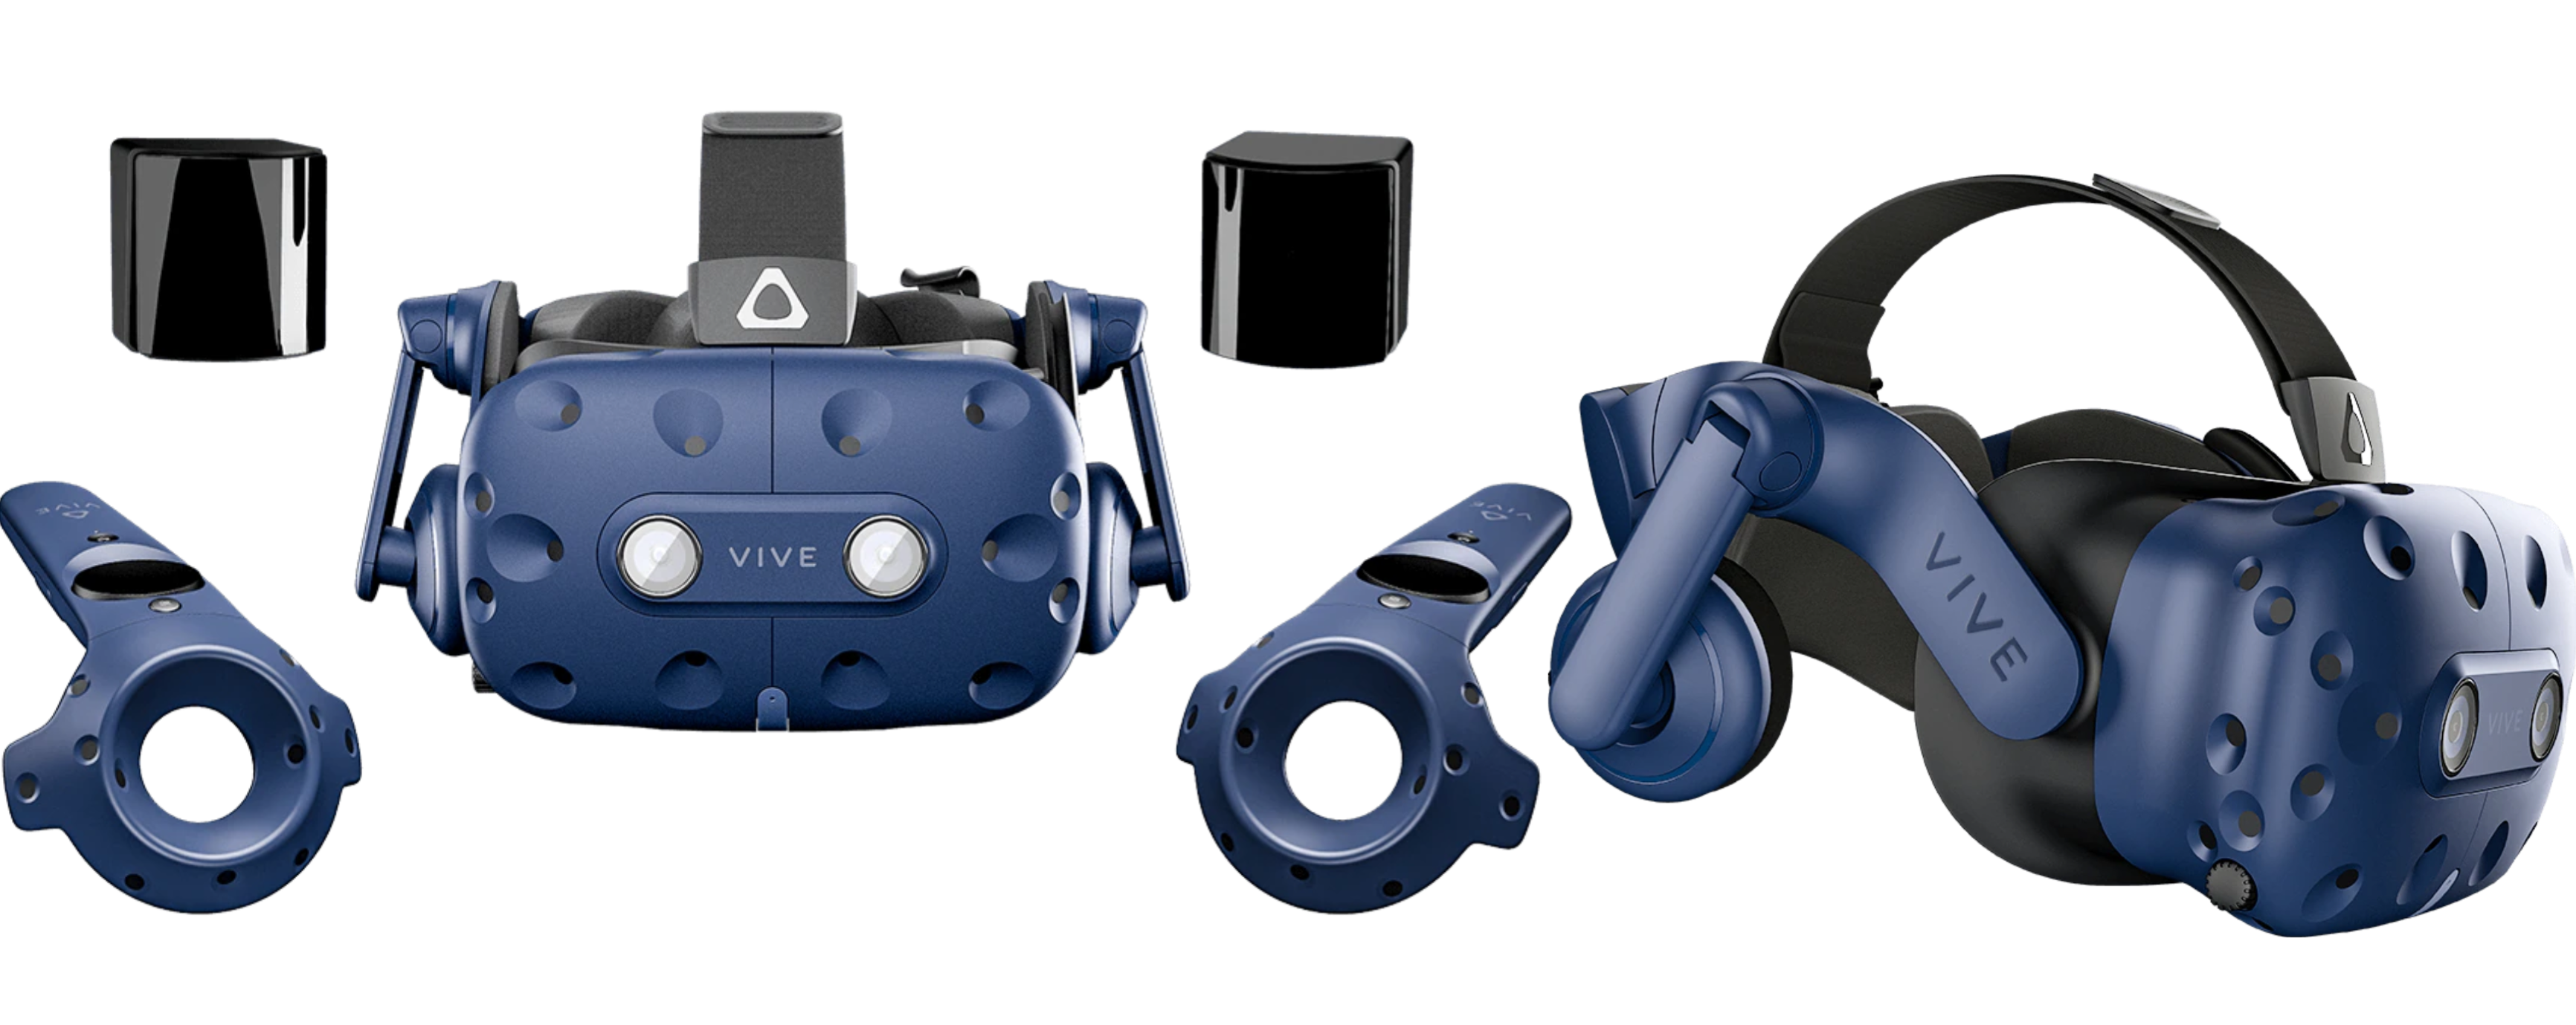
\includegraphics[width=0.7\textwidth]{images/htc_vive_pro_full.PNG}
    \caption[HTC Vive Pro]{HTC Vive Pro \cite{ViveProFullKit}}
    \label{fig:htc_vive_pro}
\end{figure}

The \ac{VR} game was developed using the SteamVR plugin version 2.8.0, which is a plugin developed by Valve Corporation that allows the Unity game engine to interact with the HTC Vive \ac{VR} headset and the Vive controllers. The SteamVR plugin provides the necessary scripts and prefabs to interact with the \ac{VR} headset and the controllers. The plugin also provides the necessary scripts to interact with the \ac{VR} camera rig, which is the main camera that is used to render the \ac{VR} scene. SteamVR uses the OpenVR SDK, which is a software development kit developed by Valve Corporation that serves as the interface between the \ac{VR} hardware and the game engine\cite{WikiOpenVR}.


\subsection{Visualization of the Elements} \label{subsec:visualization_elements}

The \ac{VR} game was developed to visualize the elements of the \ac{POP} algorithm, which are the actions, the causal links, the binding constraints, the ordering constraints, and the whole plan as a \acf{DAG}. The visualization of the elements was done using the Unity game engine, the SteamVR plugin and some external assets and scripts. The following list will discuss how each element was visualized in the \ac{VR} game:

\begin{itemize}
    \item \textbf{Actions/Operators:} \\
          The actions or the operators were visualized as children building blocks. Each action was represented as a building block with the name of the action written on the block, and the preconditions and effects of the action were written on the sides of the block. The \textit{Start()} and \textit{Finish()} actions were represented as a yellow block. New actions were represented as a green block, and existing actions were represented as a red block. When the user is creating the plan, he can create new actions, interact with them, and move them around in the scene.

          \begin{figure}[H]
              \centering
              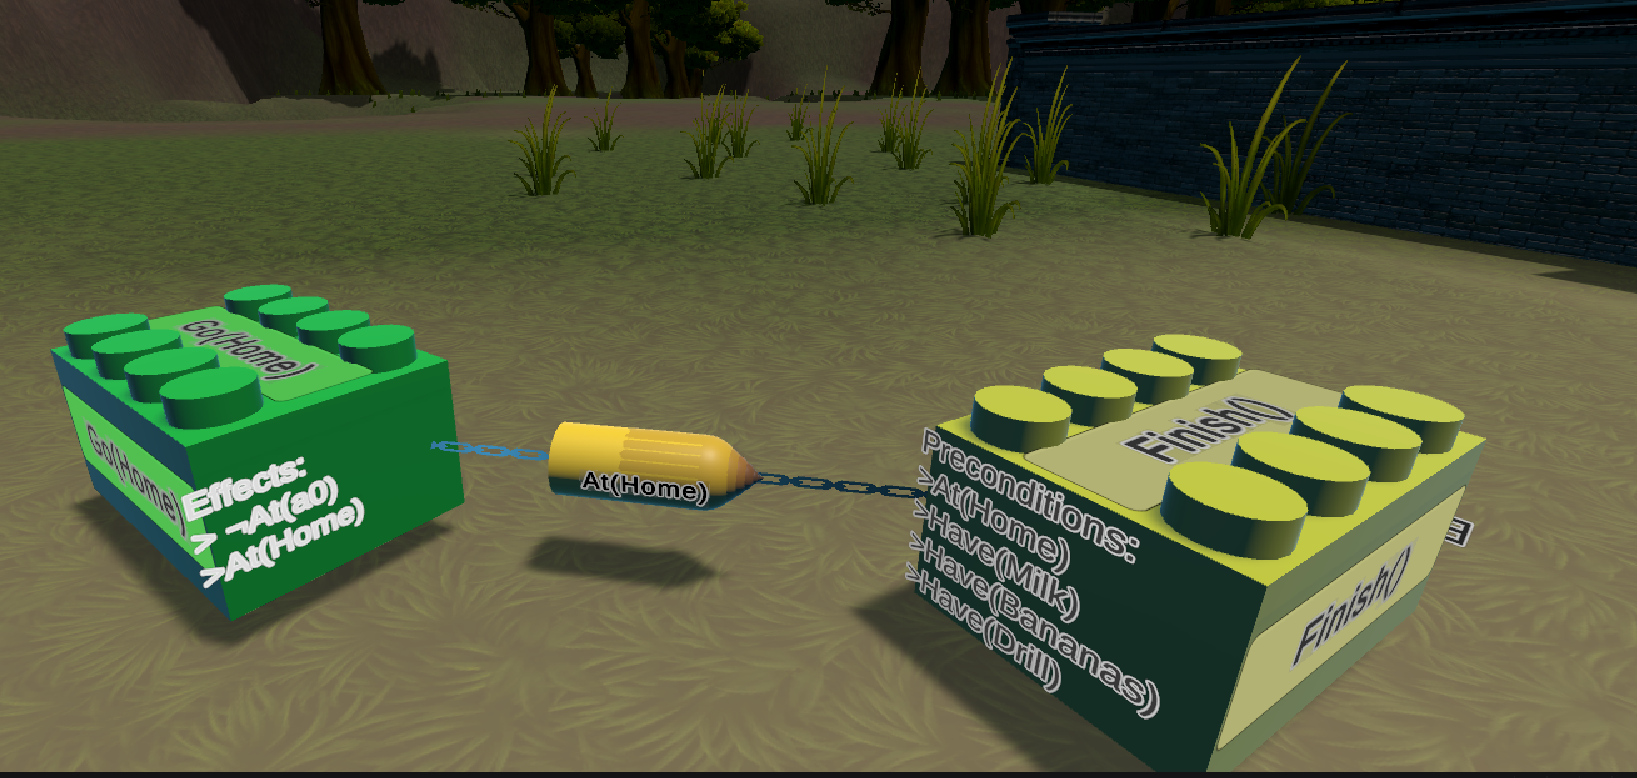
\includegraphics[width=0.9\textwidth]{images/VR_Actions_Links.png}
              \caption[Actions and Causal Links in VR]{Actions and Causal Links in VR}
              \label{fig:vr_actions_links}
          \end{figure}

    \item \textbf{Causal Links:} \\
          The causal links were visualized as lines connecting the producer action to the consumer action. The links were represented as chains with an arrow-like object in the middle of the chain that had the link conditions written on it. A link sample is shown in \autoref{fig:vr_actions_links}.

          \begin{figure}[H]
              \centering
              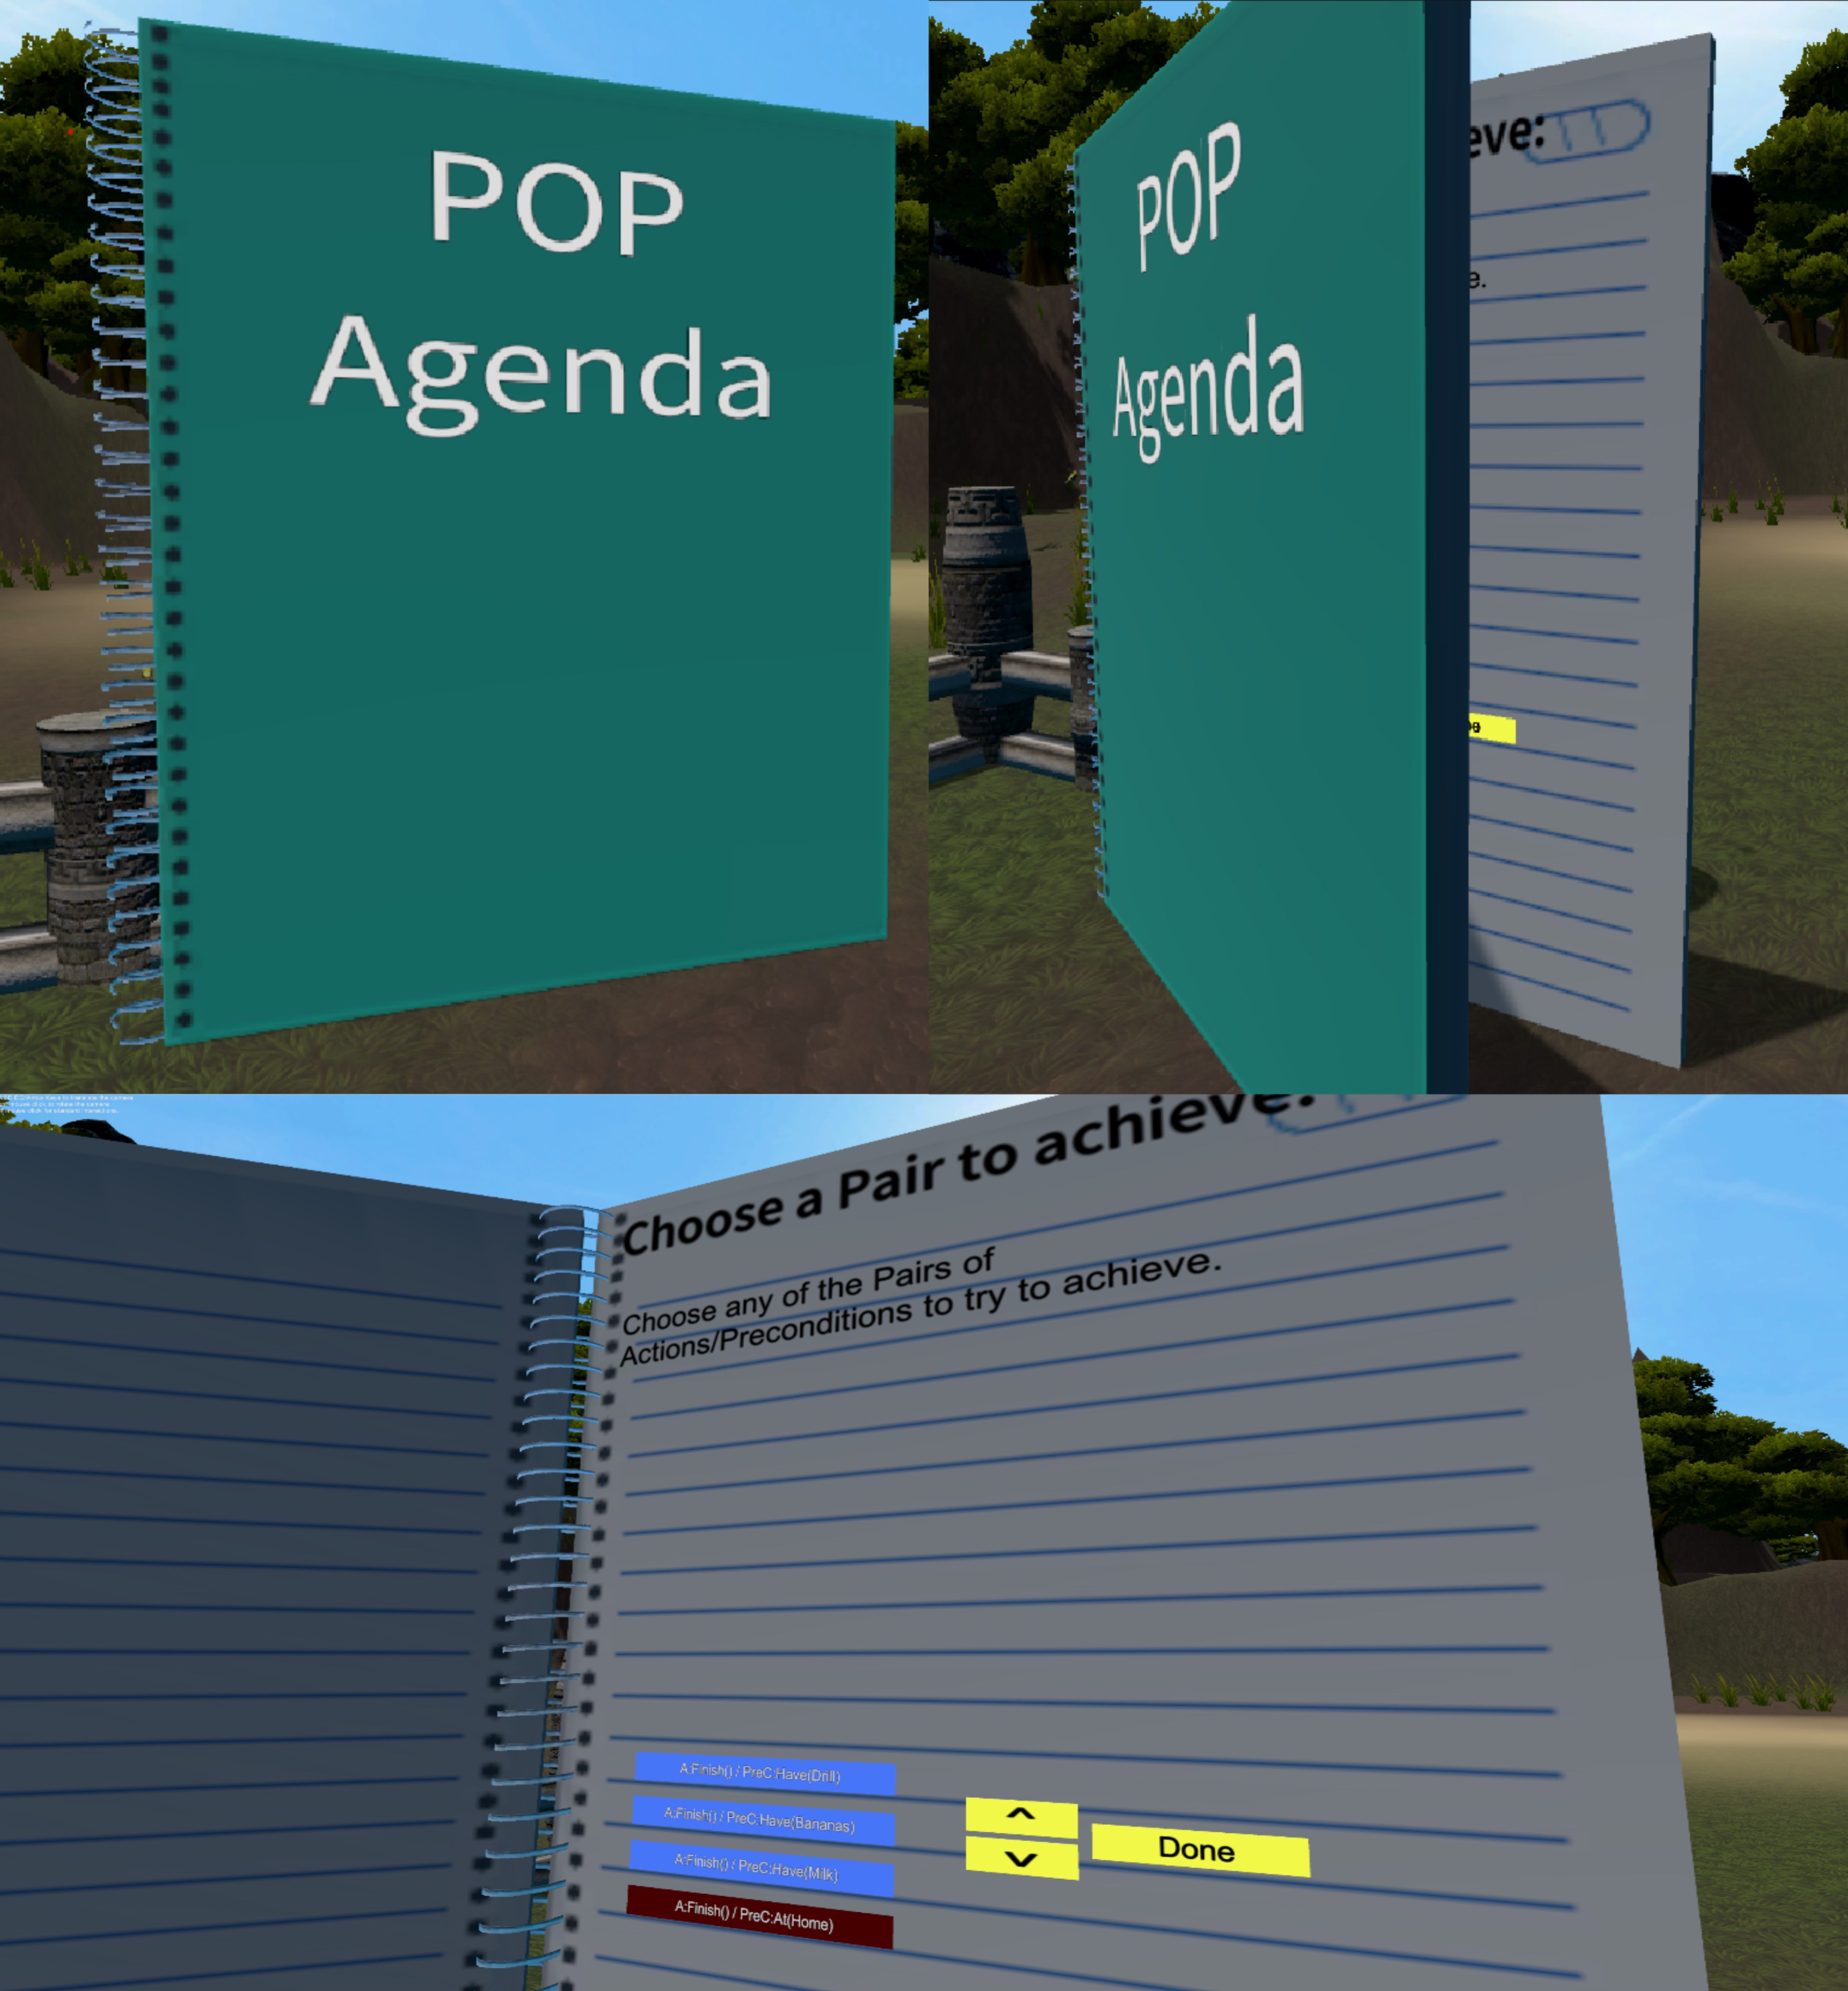
\includegraphics[width=0.5\textwidth]{images/Agenda.jpg}
              \caption[Agenda in VR]{Agenda in VR}
              \label{fig:vr_agenda}
          \end{figure}

    \item \textbf{Agenda:} \\
          The agenda was visualized as an actual agenda that the user can interact with. The agenda had the actions and the preconditions that need to be achieved. The user can interact with the agenda by selecting the action that he wants to achieve, and then it will get the list of possible achievers for this action, whether they are existing actions or new actions.

    \item \textbf{Ordering Constraints:} \\
          The ordering constraints were visualized as lines connecting the actions with a blue arrow-like object in the middle of the line that had the ordering constraints written on it. An ordering constraint sample is shown in \autoref{fig:vr_ordering_constraints}.
          \begin{figure}[H]
              \centering
              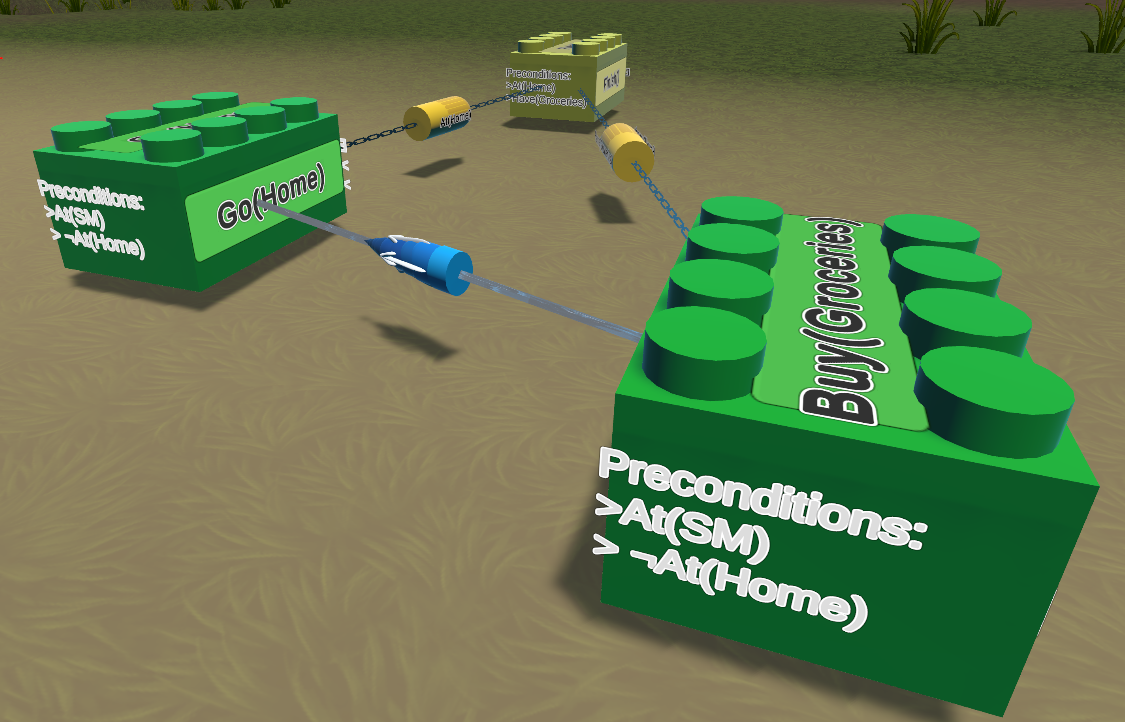
\includegraphics[width=0.3\textwidth]{images/ordering_constraints.png}
              \caption[Ordering Constraints in VR]{Ordering Constraints in VR}
              \label{fig:vr_ordering_constraints}
          \end{figure}

    \item \textbf{Threats:} \\
          The threats were always being checked in the background, and if a threat was found, the user would be notified with an emergency sound and a red alarm\cite{3DAlarmLight} light placed on a computer screen in the scene. The user can then interact with the computer screen and a keyboard to see the threats and resolve them.

          \begin{figure}[H]
              \centering
              \begin{minipage}{0.48\textwidth}
                  \centering
                  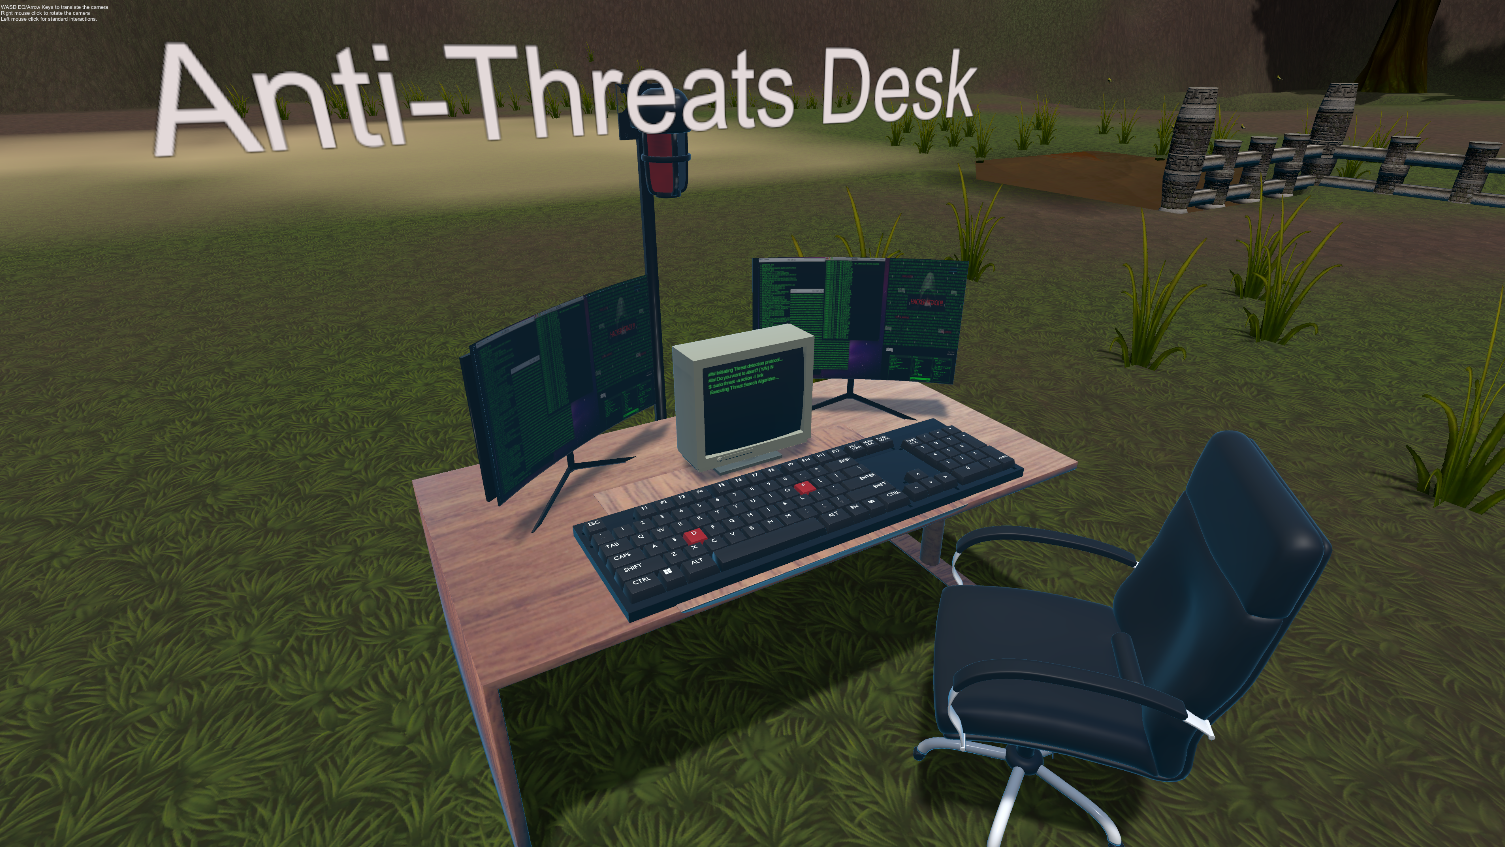
\includegraphics[width=\textwidth]{images/Threats1.png}
                  \caption[Threats in VR]{Threats Computer Desk}
                  \label{fig:vr_threats}
              \end{minipage}\hfill
              \begin{minipage}{0.48\textwidth}
                  \centering
                  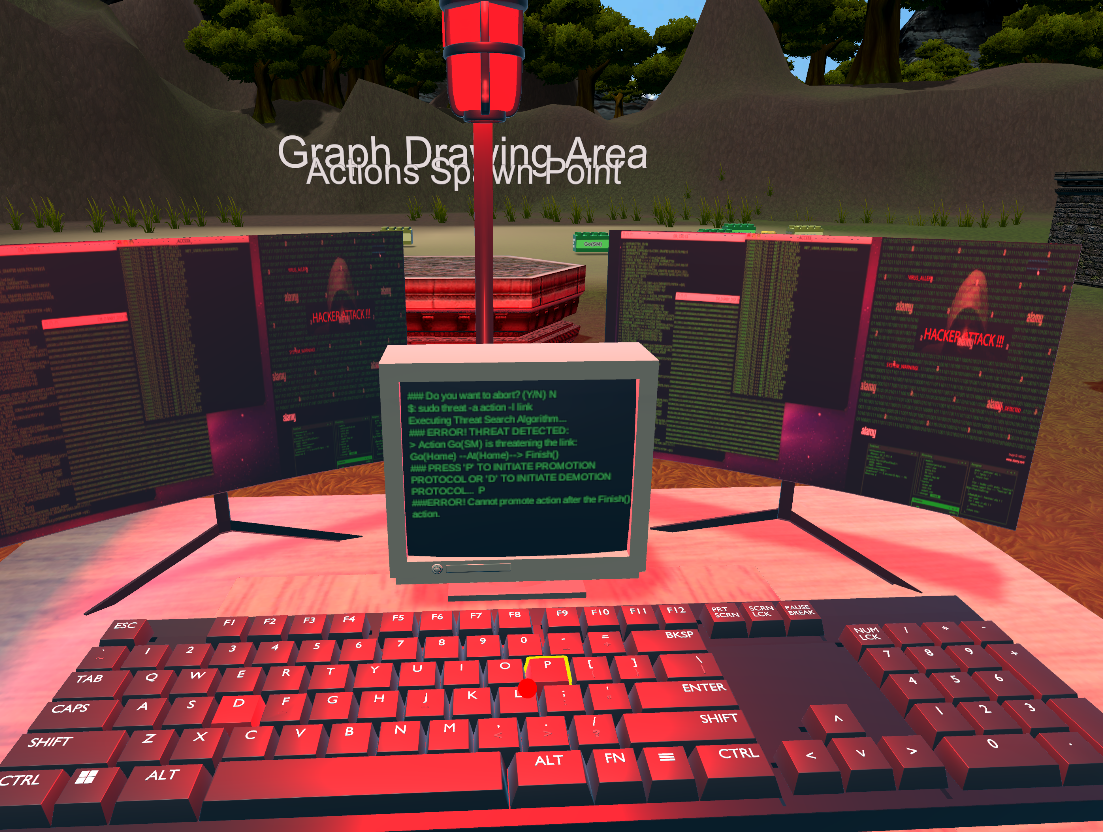
\includegraphics[width=\textwidth]{images/Threats2.png}
                  \caption[Threats in VR]{Threats Alert}
                  \label{fig:vr_threats2}
              \end{minipage}
          \end{figure}

    \item \textbf{Auto Graph Layout:} \\
          The \ac{DAG} of the plan was visualized using the \textit{Force Directed Graph} algorithm. \textit{Force Directed Graph} is an algorithm that is used to visualize graphs in a 2D or 3D space. The algorithm uses forces to simulate the physical behavior of the nodes and the edges of the graph. The algorithm was used to show the user the final plan and the intermediate steps that the planner went through as a floating graph in the scene.

          The implementation of the \textit{Force Directed Graph} algorithm was mainly inspired by the implementation in the GitHub repository, \textit{Force-Directed-Graph}, of the Ph.D. candidate, \textit{Omar Addam}, that is under the MIT license\cite{GitHubFDG}. The code was modified to fit the needs of the \ac{VR} game and the \ac{POP} algorithm, as the original implementation was visualized using a 2D view in Unity3D and was designed to use the mouse to interact with 2D image nodes. The modified implementation was designed to use the Vive controllers to interact with the 3D nodes in the \ac{VR} game and to carry all needed data to synchronize the \ac{POP} algorithm with the graph.           A snapshot of the \textit{Force Directed Graph} in the \ac{VR} game is shown in \autoref{fig:vr_dag}.

          \begin{figure}[H]
              \centering
              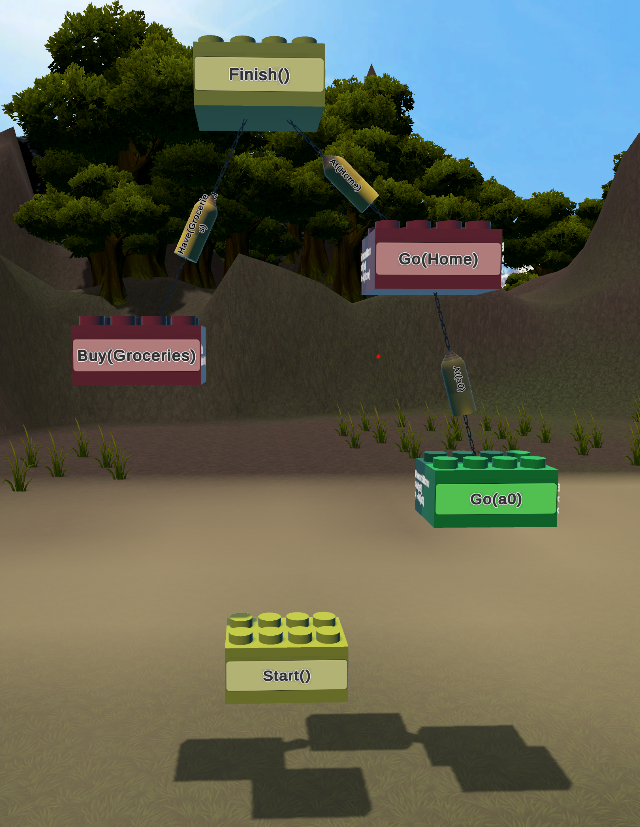
\includegraphics[width=0.5\textwidth]{images/snapshot_of_spectator.png}
              \caption[Force Directed Graph in VR]{Floating Force Directed Graph (Spectator View)}
              \label{fig:vr_dag}
          \end{figure}

    \item \textbf{Game Starting Environment:} \\
          The game starting environment was designed to look like an old temple with some ancient artifacts. The user starts the game in the temple, and then he can teleport to the different options in the game, where he can choose some properties of the planner before starting the game. The exact options that the user can choose are discussed in later sections. A top view of the game starting environment is shown in \autoref{fig:vr_pre_environment}.\\

          \begin{figure}[h]
              \centering
              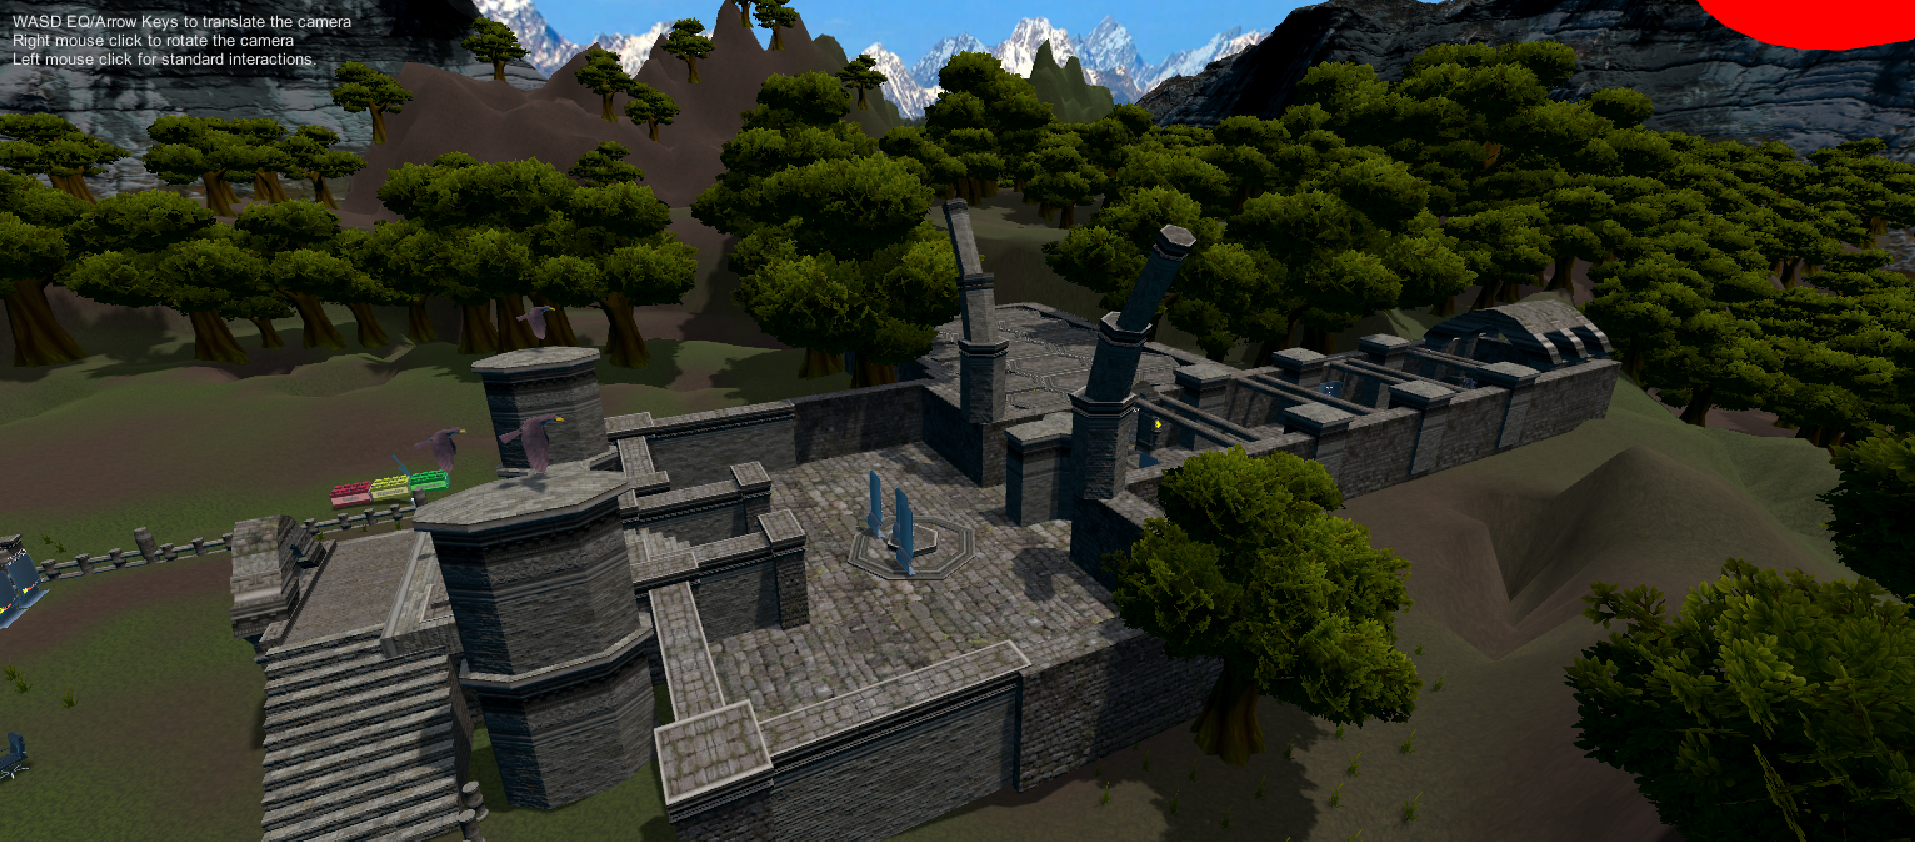
\includegraphics[width=0.8\textwidth]{images/Enviroment1.png}
              \caption[Game Starting Environment in VR]{Game Starting Environment Top View}
              \label{fig:vr_pre_environment}
          \end{figure}

    \item \textbf{Main Game Environment:} \\
          The main game environment was designed to look like a grass open area with some trees and mountains in the background. The graph area, where the user can see or even construct the plan, was marked by yellow sand color. The environment has a computer desk with a screen that shows the threats, the agenda, two menus to delete links or ordering constraints, and other options. A top view of the main game environment is shown in \autoref{fig:vr_main_environment}.

          \begin{figure}[h]%TODO take a better screenshot
              \centering
              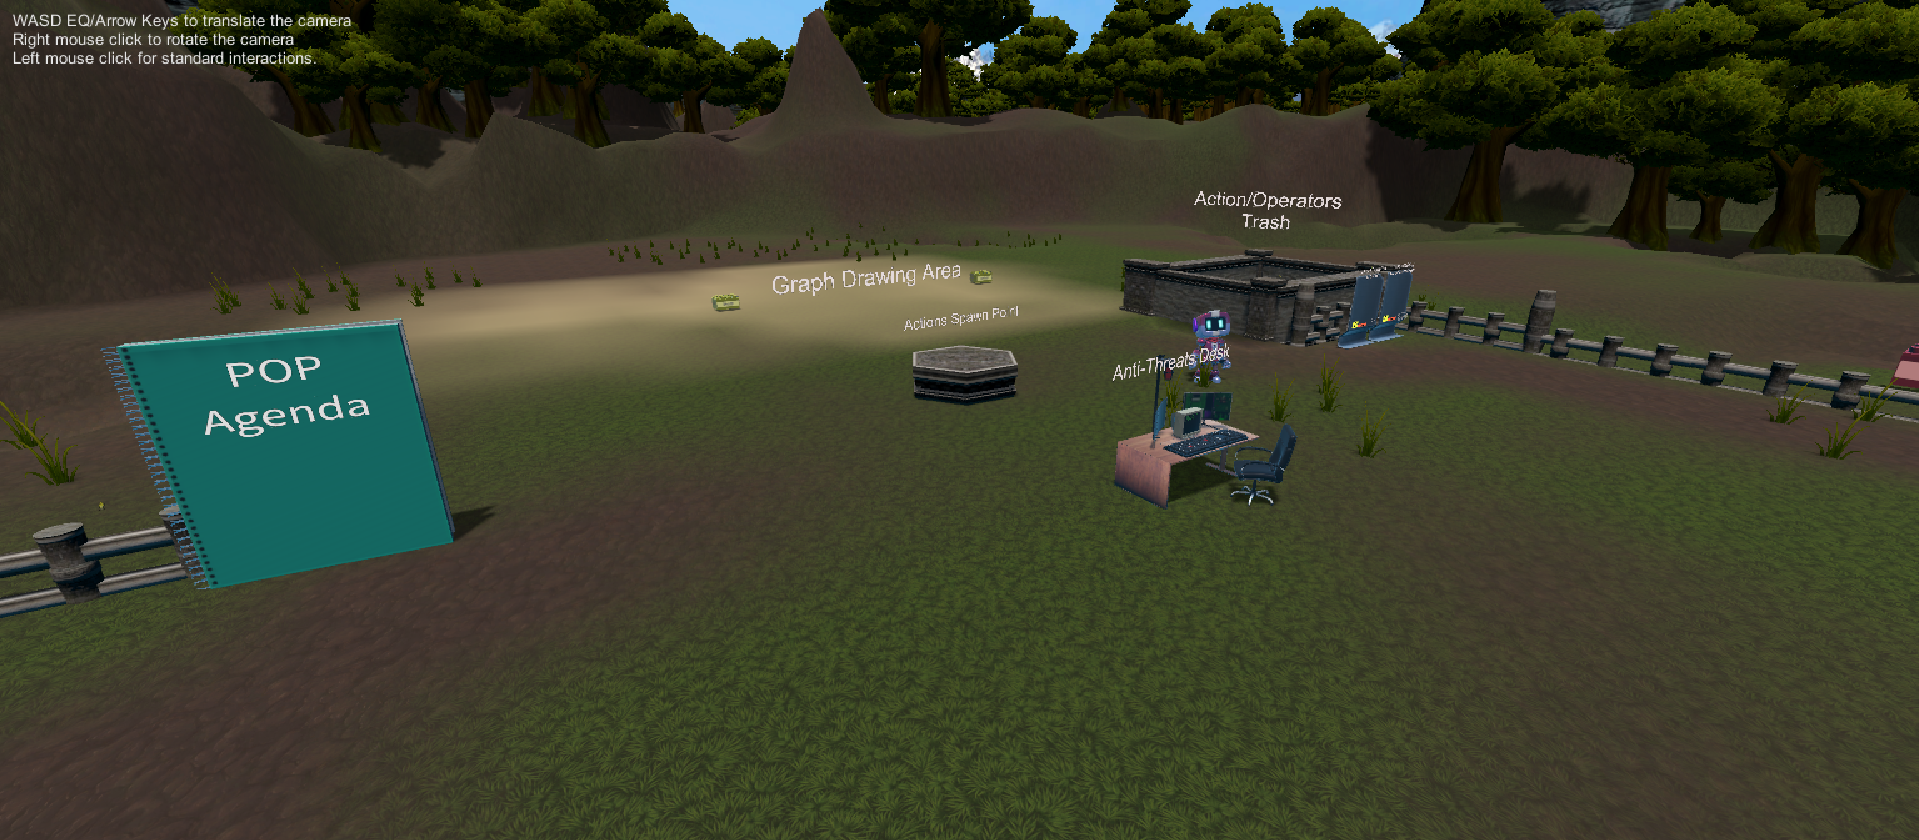
\includegraphics[width=0.8\textwidth]{images/Enviroment2.png}
              \caption[Main Game Environment in VR]{Main Game Environment Top View}
              \label{fig:vr_main_environment}
          \end{figure}
\end{itemize}


\subsection{User Interaction} \label{subsec:user_interaction}
The user can interact with the \ac{VR} game using the HTC Vive controllers or the mouse and the keyboard in case of using a simulated \ac{VR} environment. The main interactions that the user can do in the game are as follows:

\begin{itemize}
    \item \textbf{Teleportation:} \\
          The user can teleport to different locations in the game by pressing the touchpad of the Vive controller. The user can point anywhere, where teleport markers are put in the game, then leave the teleport button to teleport there. The teleportation was implemented using the SteamVR plugin. In the case of using the simulated \ac{VR} environment, the user can either use the arrow keys to move around or use the button \textit{T} to mimic the Vive controller teleportation.

    \item \textbf{Interacting with Buttons:} \\
          The user can interact with buttons in the game by approaching the button and pressing the trigger button of the Vive controller when the button is highlighted. In the case of using the simulated \ac{VR} environment, the user can use the mouse to click on the buttons.

    \item \textbf{Interacting with Interactables:} \\
          The user can interact interactables in the game by approaching the interactable and pressing the trigger button of the Vive controller when the interactable is highlighted. If the interactable can be held or moved, the user can hold the trigger button and move the interactable around in the scene. Usually, there are limitations from the SteamVR plugin that the user cannot hold the interactable and teleport at the same time, so the user can simply hold the interactable with one controller and teleport with the other. In the case of using the simulated \ac{VR} environment, the user can use the mouse to click on the interactables and drag them around. The right mouse button can be used to rotate the camera view.
\end{itemize}

\subsection{Game Walkthrough} \label{subsec:game_walkthrough}
This section will discuss the walkthrough of the \ac{VR} game, the options that the user can choose, how the user can interact with the game, and how the game can guide the user. This section will also discuss the different modes that the user can choose to interact with the graph.

\subsubsection{User Path Guidance} \label{subsubsec:user_path_guidance}
When the user starts the game, he is guided to the temple environment, where he can choose some options before starting the game. The user is guided to the temple environment by a path of green arrows that are placed on the ground. The green arrows are placed in the direction that the user should follow to reach the next step in the game. The arrows guide are shown when the user presses the teleport button of the Vive controller, and they disappear when the user releases the teleport button. The main environment also has some green arrows that guide the user to the agenda, the threats and so on. There are also some yellow arrows that indicate an optional path.

\begin{figure}[H]
    \centering
    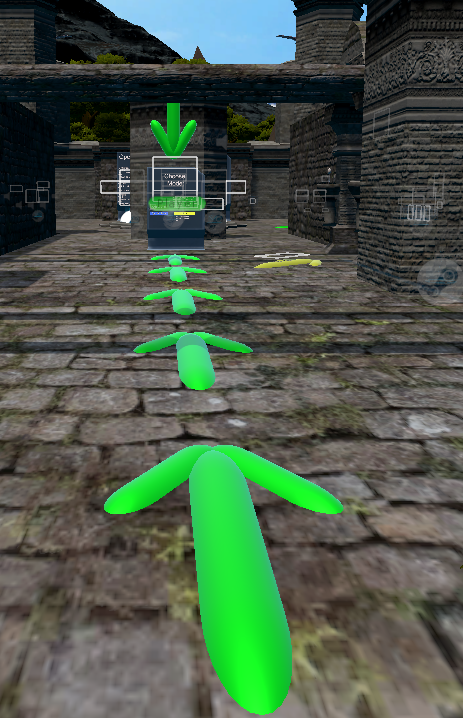
\includegraphics[width=0.45\textwidth]{images/user_guide.png}
    \caption[User Path Guidance in VR]{User Path Guidance in the Environment}
    \label{fig:vr_user_guide}
\end{figure}

\subsubsection{Pre-Game Options} \label{subsubsec:pre_game_options}

The user starts the game in the temple environment, where he can choose some options before starting the game. This stage is called the \textit{Pre-Game Options}. The user can choose the following options:

\begin{itemize}
    \begin{figure}[H]
        \centering
        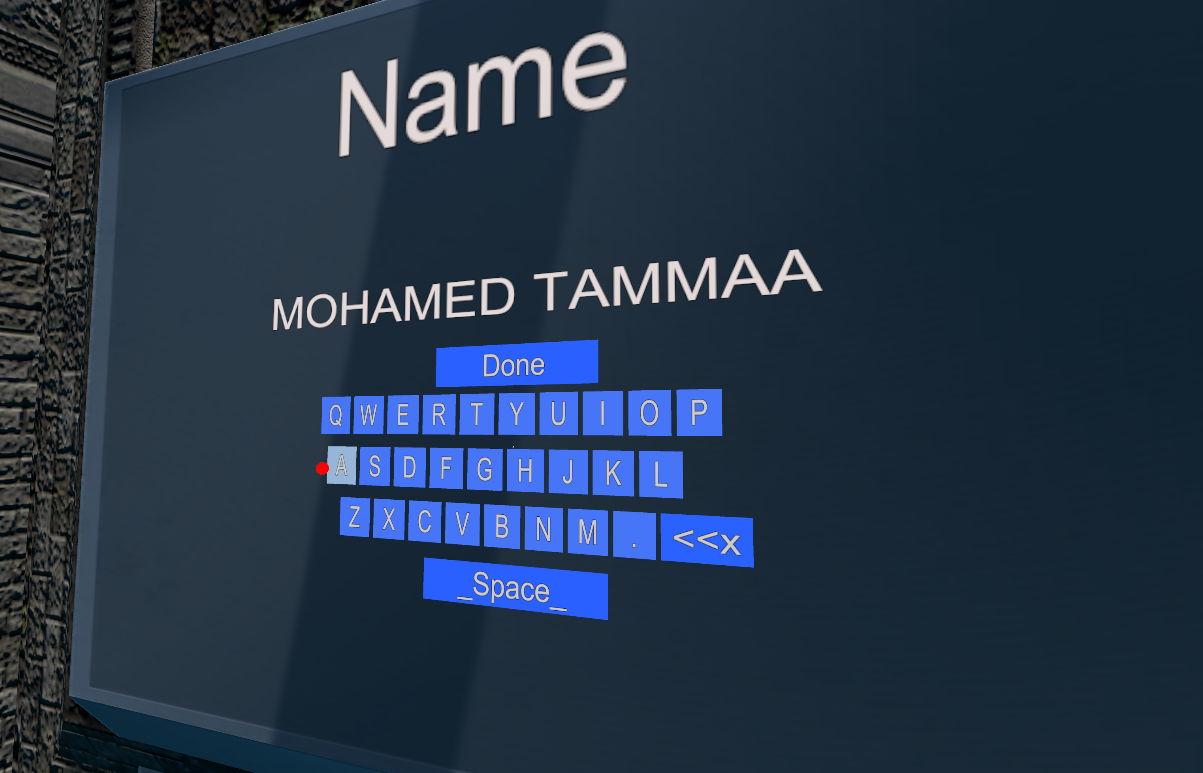
\includegraphics[width=0.6\textwidth]{images/name_menu.png}
        \caption[Name Entering Menu in VR]{Name Entering Menu in VR}
        \label{fig:vr_name_entering_menu}
    \end{figure}
    \item \textbf{Name Entering Menu:} \\
          The first menu that the user encounters is the \textit{Name Entering Menu}, where the user can enter his name. The user can enter his name using the keyboard that is placed in front of him inside the scene. The user can then press the \textit{Done} button to save his name.

          \begin{figure}[H]
              \centering
              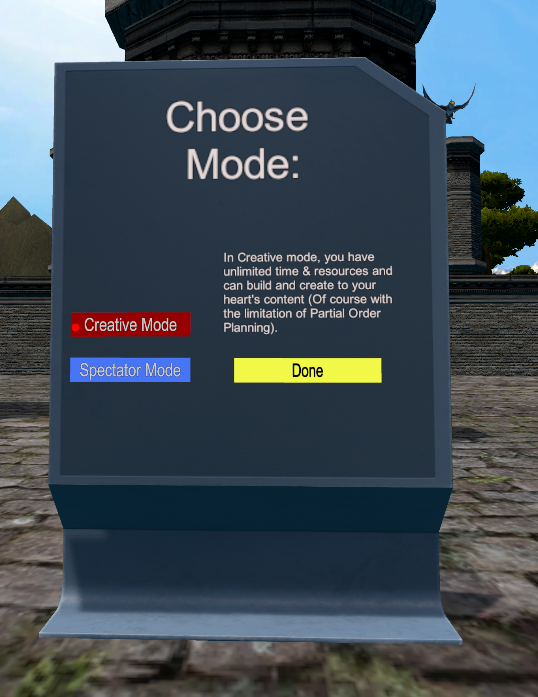
\includegraphics[width=0.4\textwidth]{images/mode_menu.png}
              \caption[Mode Selection Menu in VR]{Mode Selection Menu}
              \label{fig:vr_mode_selection_menu}
          \end{figure}


    \item \textbf{Mode Selection Menu:} \\
          The second menu that the user encounters is the \textit{Mode Selection Menu}, where the user can choose the mode that he wants to play in. The user can choose between the \textit{Creative Mode} and the \textit{Spectator Mode}.

          The \textit{Creative Mode} allows the user to be the planner, where he can check the agenda, create new actions and delete them, create new causal links and delete them, and check the threats and resolve them. The user has full control over the planner in this mode, while given some guidance from the planner, helping with the bindings and suggesting achievers.

          The \textit{Spectator Mode} allows the user to watch the planner working on the plan, applying achievers, resolving threats, backtracking from wrong decisions, and finally finding the optimal plan. The user can only watch the planner in this mode, and the only interactions that the user can do are starting or pausing the planner to check the new steps, and teleporting around the scene to see the plan from different angles.

    \item \textbf{Planning Problem Selection Menu:} \\
          The third menu that the user sees is the \textit{Planning Problem Selection Menu}, where the user can choose the planning problem that he wants to solve or watch the planner solving. The user can choose between the \textit{Socks and Shoes problem}, the \textit{Milk, Bananas, and Cordless Drill problem}, the \textit{Groceries Buying problem} and the \textit{Spare Tires problem}. When the user chooses the planning problem, the initial state, the goal state, and the operators of the problem with their preconditions and effects are shown to the user to the right and left of the \textit{Planning Problem Menu}. The user can explore the problem and understand it before starting the planner.

          \begin{figure}[H]
              \centering
              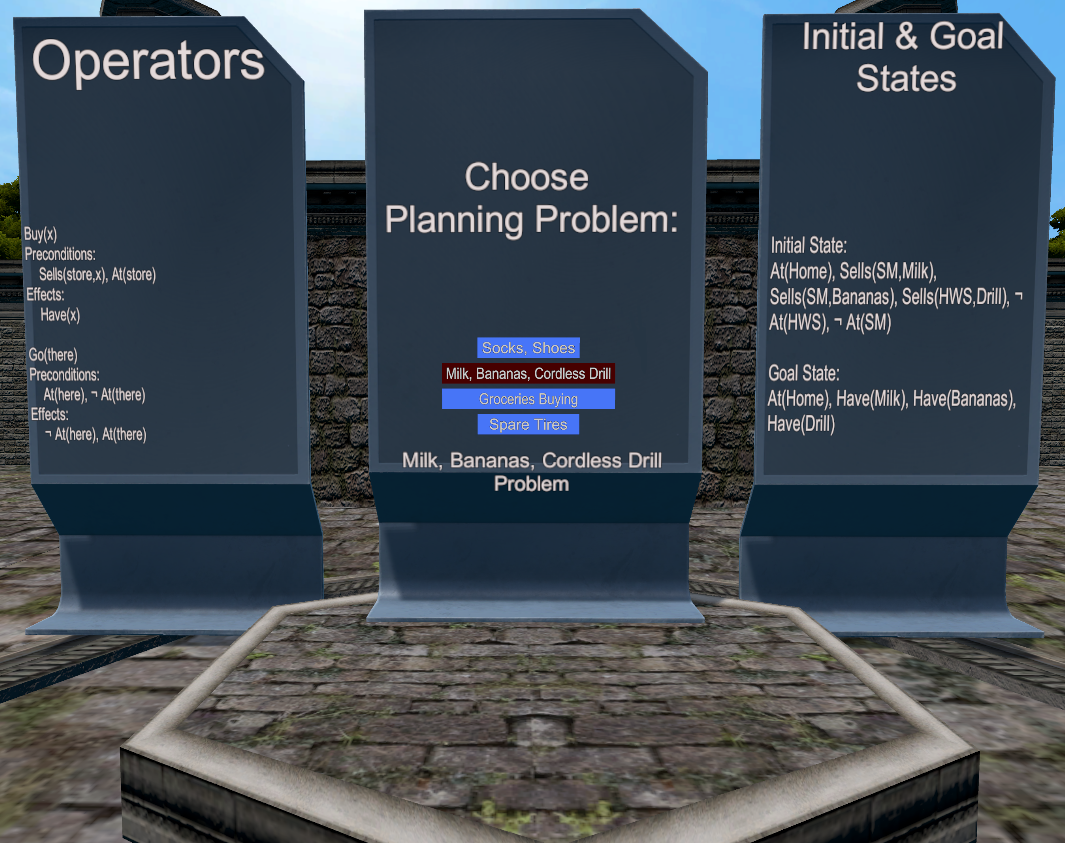
\includegraphics[width=0.7\textwidth]{images/planning_problem.png}
              \caption[Planning Problem Selection Menu in VR]{Planning Problem Selection Menu}
              \label{fig:vr_problem_selection_menu}
          \end{figure}

    \item \textbf{Search Algorithm Selection Menu:} \\
          The fourth menu that the user sees \textbf{if he chooses the \textit{Spectator Mode}} is the \textit{Search Algorithm Selection Menu}, where the user can choose the search algorithm that he wants to watch the planner using it. The user can choose between \textit{\ac{DFS}}, \textit{\ac{BFS}} and \textit{\ac{A*} Search}. The user see a brief explanation of each search algorithm and how it works. The user can then choose the search algorithm that he wants to watch the planner using it. If the user chooses the \textit{\ac{DFS}}, another menu will appear and the user will be asked to enter the maximum depth of the search tree that the planner can go through. Entering the maximum depth is important to avoid infinite loops in the search tree. Moreover, the game will suggest a maximum depth based on the planning problem that the user chose.

          \begin{figure}[H]
              \centering
              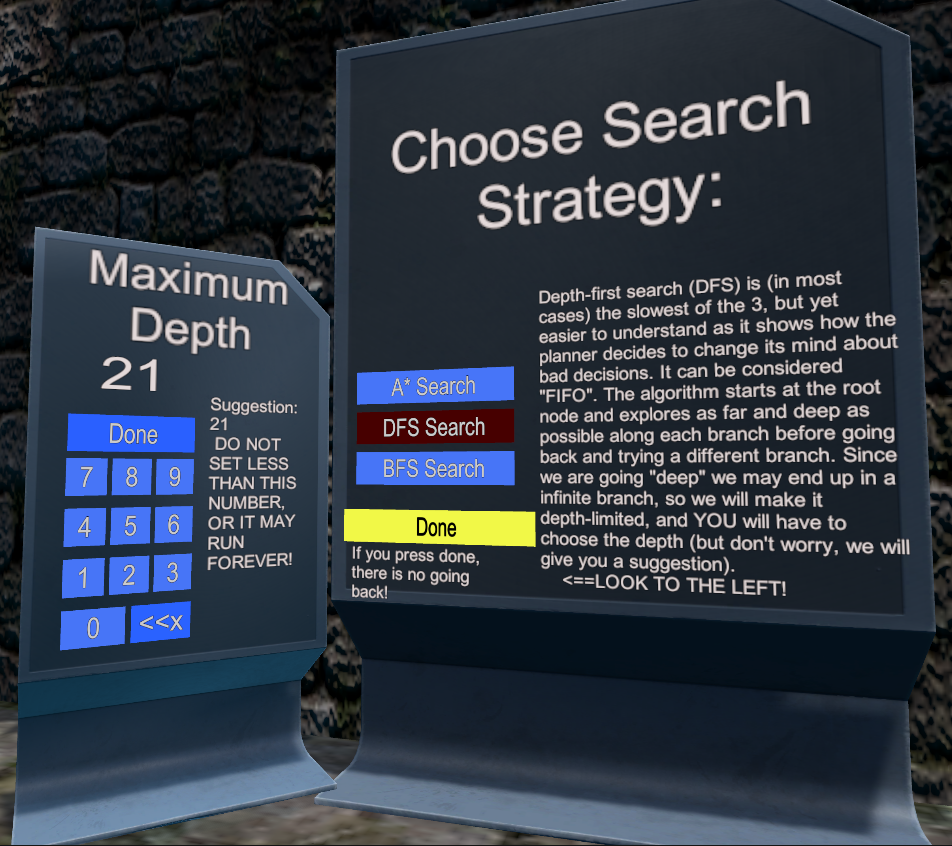
\includegraphics[width=0.6\textwidth]{images/search_strategy.png}
              \caption[Search Algorithm Selection Menu in VR]{Search Algorithm Selection Menu in VR}
              \label{fig:vr_search_algorithm_menu}
          \end{figure}

    \item \textbf{Ready to Start Menu:} \\
          The last menu that the user sees before starting the game is that he is asked if he is ready to start the planner. When the user confirms that he is ready, the game will start and the planner will start working on the plan, or initializes the environment for the user to start planning.

\end{itemize}

\subsubsection{Spectator Game Environment} \label{subsubsec:spectator_game_environment}
The user is instructed to go to the main game environment, where he can watch the planner working on the plan. The user can teleport around the scene to see the plan.
There are two buttons used in the \textit{Vive Controller} to interact with the planner:

\begin{figure}[H]
    \centering
    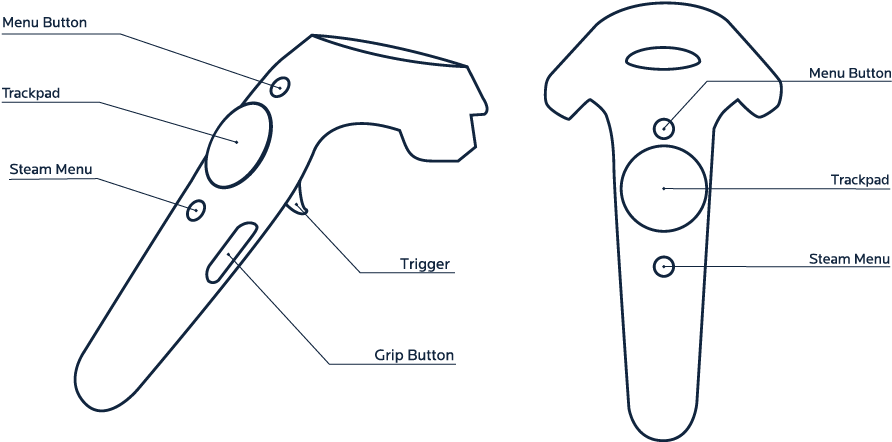
\includegraphics[width=0.7\textwidth]{images/vive_controller.png}
    \caption[Vive Controller]{Vive Controller\cite{UE4ViveController}}
    \label{fig:vive_controller}
\end{figure}

\begin{itemize}
    \item \textbf{Menu Button:} \\
          The user can press the menu button of the Vive controller to let the planner show the next step of the plan. After the planner shows the next step, it will stop and wait for the user to press the menu button again to show the next step.

    \item \textbf{Grip Button:} \\
          The user can press the grip button of the Vive controller to shuffle the graph nodes. The reason why the user can shuffle the graph nodes is to avoid the nodes or edges from overlapping each other, as the \textit{Force Directed Graph} algorithm may not always give the best layout of the graph. The user can press the grip button multiple times to shuffle the graph nodes until he gets a better layout of the graph.
\end{itemize}


\subsubsection{Creative Game Environment} \label{subsubsec:creative_game_environment}
When the user chooses the \textit{Creative Mode}, he is instructed to go to the main game environment, where he can start planning. The user can check the agenda, create new actions, throw actions in the trash and delete them, create new causal links, delete causal links and ordering constraints, check the threats, and resolve the threats. The user can also interact with the graph and move the nodes around to get a better layout of the graph. In this mode, the graph is not floating in the scene, but it is placed on the yellow sand area in the scene to be more easier for the user to interact with the graph. The following list will discuss the interactions that the user can do in the \textit{Creative Mode}:

\begin{itemize}
    \item \textbf{Agenda:} \\
          The user can check the agenda by approaching the agenda and then the agenda will automatically open. The user can then select the pair of action and preconditions that he wants to achieve, and then the planner will suggest the possible achievers for this action. The user can then choose between creating a new action or selecting an existing action to achieve the preconditions. The agenda will give the feedback to the user if he chose an existing action that cannot unify or bind the preconditions, or if he chose to link an action that will cause the graph to have a cycle. (See \autoref{fig:vr_agenda})

    \item \textbf{Actions Spawn Point} \\
          If the user chooses to create a new action as an achiever for the preconditions, he can go to the \textit{Actions Spawn Point} where the new action will fall from the sky. The user is then asked to take the action and place it in the graph for it to be linked automatically. The user can then move the action around in the scene, or throw it in the trash if he does not want to use it. (See \autoref{fig:vr_actions_spawn_point})


    \item \textbf{Trash:} \\
          If the user wants to delete an action, he can go to the \textit{Trash} and throw the action in the trash. The action will then be deleted from the graph. If the user decides to delete an action that has causal links, the causal links will also be deleted. The \textit{Start()} and \textit{Finish()} actions will be respawned back in the scene if they are thrown in the trash, as they are essential for the planner to work. (See \autoref{fig:vr_trash})
          \begin{figure}[h]
              \centering
              \begin{minipage}{0.4\textwidth}
                  \centering
                  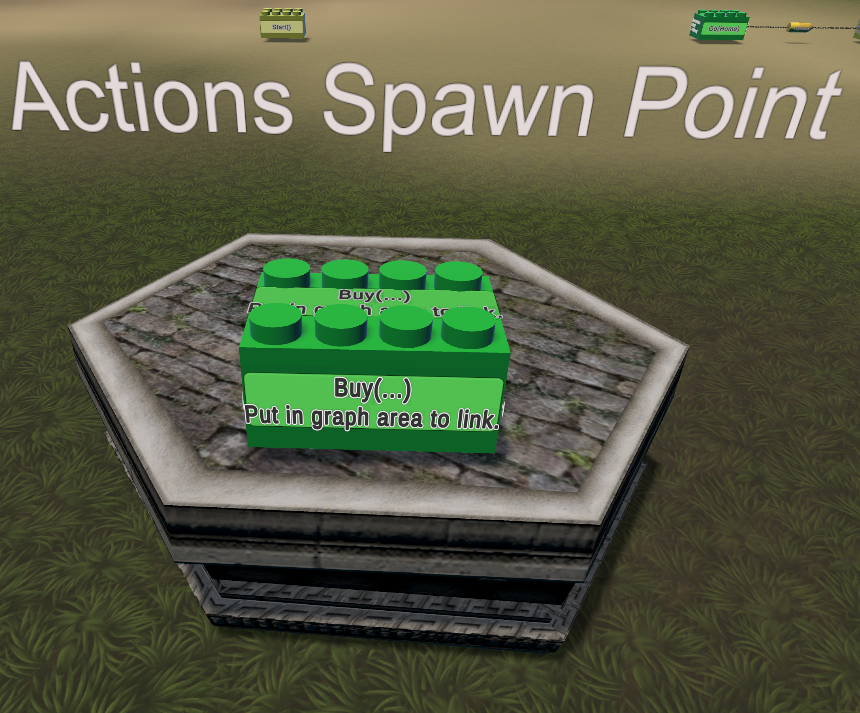
\includegraphics[width=\textwidth]{images/actions_spawn.png}
                  \caption[Actions Spawn Point in VR]{Actions Spawn Point}
                  \label{fig:vr_actions_spawn_point}
              \end{minipage}\hfill
              \begin{minipage}{0.4\textwidth}
                  \centering
                  \includegraphics[width=\textwidth]{images/trash.png}
                  \caption[Trash in VR]{Actions Trash}
                  \label{fig:vr_trash}
              \end{minipage}
          \end{figure}

    \item \textbf{Causal Links and Ordering Constraints Deletion:} \\
          The user can delete causal links and ordering constraints by going to any of the causal links or ordering constraints menus and selecting the link or constraint that he wants to delete. The user can then press the delete button to delete the link or constraint. (See \autoref{fig:vr_causal_links_ordering_constraints_menu})

          \begin{figure}[h]
              \centering
              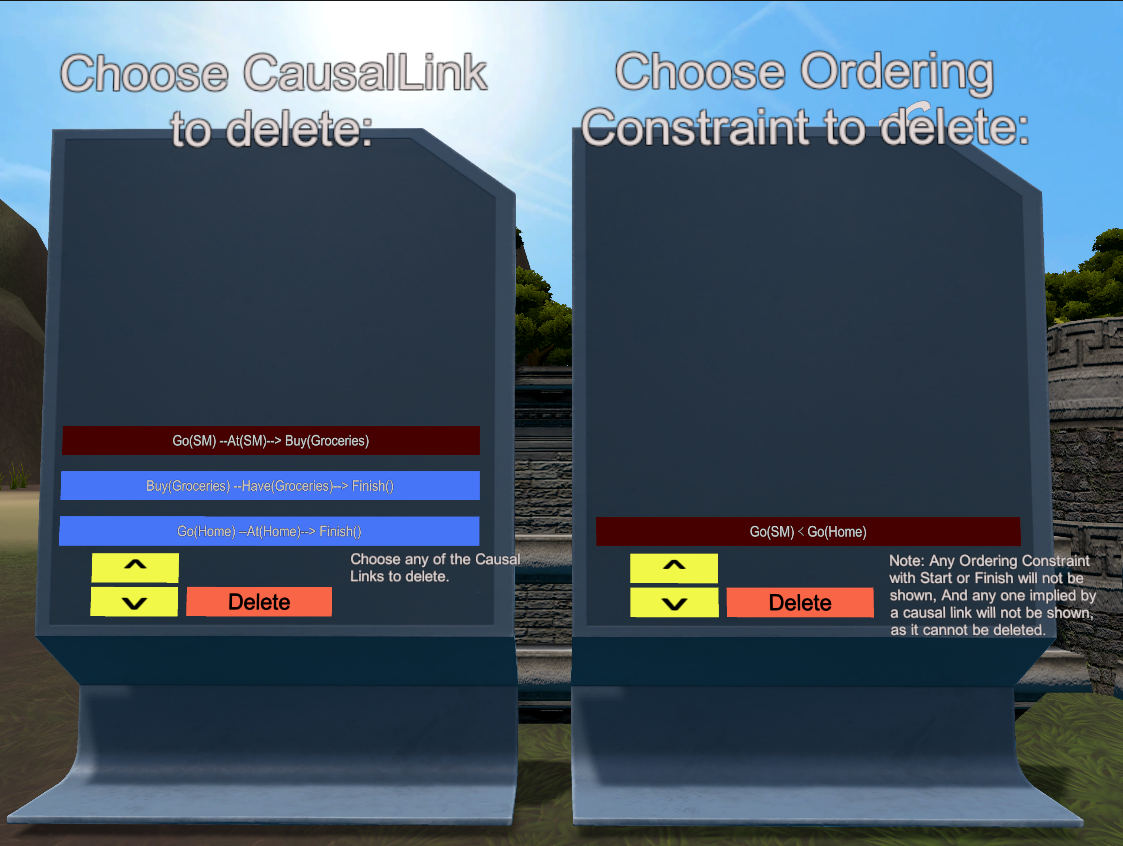
\includegraphics[width=0.6\textwidth]{images/delete_links_order.png}
              \caption[Causal Links and Ordering Constraints Menu in VR]{Causal Links and Ordering Constraints Menu}
              \label{fig:vr_causal_links_ordering_constraints_menu}
          \end{figure}

    \item \textbf{Threats Desk:} \\
          When the user is notified with a threat, he can go to the \textit{Threats Desk} and interact with the computer screen to see the threats and resolve them. The user is notified with an emergency sound and a red alarm light placed on the computer desk. The user is asked to resolve the threats before continuing with the planner. All agenda actions will be disabled until the threats are resolved. There are four ways to resolve the threats, the user can either delete the action that causes the threat, delete the causal link that causes the threat, promote the action that is threatening the link, or demote the action that is threatened by the link. The user can use the in-game keyboard to either press \textit{P} to promote the action or \textit{D} to demote the action.
          (See Figures \ref{fig:vr_threats} and \ref{fig:vr_threats2})


\end{itemize}
